% Edit only the text between matching begin and end lines.
\documentclass[11pt,a4paper]{article}
% Shared preamble for TMUA worked solutions. Local edits here are overwritten.

% Reproducible PDFs: no timestamps, no trailer id, no build-path details.
\ifdefined\pdfsuppressptexinfo
  \pdfsuppressptexinfo=-1
  \pdfinfoomitdate=1
  \pdftrailerid{}
\fi

\usepackage{graphicx}
\usepackage{mathtools}
\usepackage{amssymb}
\usepackage{amsmath}
\usepackage{amsthm}
\usepackage{enumitem}
\usepackage{microtype}
\usepackage[table]{xcolor}
\usepackage{array}
\usepackage{booktabs}
\usepackage{tabularx}
\usepackage{longtable}
\usepackage{ragged2e}
\usepackage{fancyhdr}
\usepackage{etoolbox}
\usepackage[
  a4paper,
  left=0.8in,
  right=1in,
  top=1in,
  bottom=0.5in,
  headheight=14pt,
  headsep=0.4in
]{geometry}

\usepackage{pgfplots}
\pgfplotsset{compat=1.18}
\usepgfplotslibrary{fillbetween, polar}
\usetikzlibrary{calc, positioning}
\usetikzlibrary{angles, quotes}
\usetikzlibrary{arrows.meta}
\usetikzlibrary{decorations.pathreplacing, decorations.markings}
\usetikzlibrary{patterns}
\usetikzlibrary{intersections}

\usepackage{tocloft}
\usepackage[hidelinks]{hyperref}
\hypersetup{pdfauthor={danieljsmith.org}, pdfcreator={}, pdfsubject={}, pdfkeywords={}}
\urlstyle{same}
\tocloftpagestyle{djssolutions}
\setlength{\cftbeforesubsecskip}{2pt}
\setlength{\cftsubsecindent}{1.5em}
\setlength{\cftsubsecnumwidth}{0pt}
\renewcommand{\cftsubsecfont}{\small\color{black}}
\renewcommand{\cftsubsecpagefont}{\small\color{black}}
\renewcommand{\cftsubsecleader}{\hfill}

% `most` carries the breakable and enhanced libraries the solution box needs.
\usepackage[most]{tcolorbox}
\definecolor{scarlet}{RGB}{205, 40, 75}

\setlength{\parindent}{0pt}

% \djsSolutionsSetup{<paper title>}, called once after this file.
\newcommand{\djsSolnPaperTitle}{}
\newcommand{\djsSolutionsSetup}[1]{%
  \hypersetup{pdftitle={#1 Solutions}}%
  \renewcommand{\djsSolnPaperTitle}{#1}}

% \djsTitleSetup{<booklet>}{<title>}{<paper name>}{<questions>}{<minutes>},
% called once after the setup line, sets the title block that opens the
% contents page, as on the question paper: TMUA and the booklet in spaced
% burgundy capitals, the title, a hairline led by the solution box's short
% scarlet rule, then the paper's name with the question count and, when
% given, the time allowed. Its colours are the site's accent, rule and muted
% text colours.
\definecolor{djsBurgundy}{RGB}{118, 59, 67}
\definecolor{djsHairline}{RGB}{216, 213, 205}
\definecolor{djsSlash}{RGB}{170, 166, 158}
\definecolor{djsMuted}{RGB}{96, 101, 106}
\makeatletter
\newcommand{\djs@booklet}{}
\newcommand{\djs@title}{}
\newcommand{\djs@papername}{}
\newcommand{\djs@details}{}
\newcommand{\djs@caps}[1]{\textls[180]{\MakeUppercase{#1}}}
\newcommand{\djs@dot}{\hspace{0.45em}\textperiodcentered\hspace{0.45em}}
\newcommand{\djsTitleSetup}[5]{%
  \renewcommand{\djs@booklet}{#1}%
  \renewcommand{\djs@title}{#2}%
  \renewcommand{\djs@papername}{#3}%
  \renewcommand{\djs@details}{%
    #4~question\ifnum#4=1 \else s\fi
    \ifblank{#5}{}{\djs@dot#5~minutes}}}
\newcommand{\djsContentsTitle}{%
  {\raggedright\color{djsBurgundy}\footnotesize\bfseries
    \djs@caps{TMUA}{\color{djsSlash}\hspace{0.55em}/\hspace{0.55em}}%
    \djs@caps{\djs@booklet}\par}%
  \vspace{7pt}%
  {\raggedright\fontsize{24.88}{28}\selectfont\djs@title\par}%
  \vspace{9pt}%
  \noindent\makebox[0pt][l]{\color{djsHairline}\rule[0.9pt]{\linewidth}{0.6pt}}%
  {\color{scarlet}\rule{3.5cm}{2.2pt}}\par
  \vspace{5pt}%
  {\small\color{djsMuted}\djs@papername\hfill\djs@details\par}%
  \vspace{8pt}}
\makeatother

% The header appears only on the contents page and each question's opening
% page. Continuation pages use the empty default style.
\fancypagestyle{djssolutions}{%
  \fancyhead{}%
  \fancyfoot{}%
  \renewcommand{\headrulewidth}{0.9pt}%
  \fancyhead[L]{\textit{Solutions} - \djsSolnPaperTitle}%
  \fancyhead[R]{\href{https://danieljsmith.org/?utm_source=pdf&utm_campaign=tmua&utm_content=solutions}{danieljsmith.org}}%
}
\pagestyle{empty}

% \djsLastUpdated{<date>}, called once after the setup line: one line
% at the foot of the first page only, left-aligned under the left header at
% the 0.8in left margin. It is drawn over the page rather than set as a
% footer, so no page style changes.
\newcommand{\djsLastUpdated}[1]{%
  \AtBeginDocument{\AddToHookNext{shipout/foreground}{%
    \put(0.8in,-\dimexpr\paperheight-0.32in\relax){\makebox[0pt][l]{%
      \footnotesize Last updated #1}}}}}

\newcolumntype{Y}{>{\RaggedRight\arraybackslash}X}

% Question layout, identical to the question paper's.
\newcommand{\djsTocTopic}[1]{%
  \ifblank{#1}{}{%
    \texorpdfstring
      {\hspace{0.9em}{\footnotesize\itshape\color{black!45}#1}}
      { \textendash\ #1}}}
\newcommand{\djsTopicLine}[1]{%
  \ifblank{#1}{}{%
    {\raggedleft\footnotesize\itshape\color{black!45}#1\par}%
    \vspace{-0.6\baselineskip}}}
\newcommand{\questionitem}[1][]{%
  \item\phantomsection
  \addcontentsline{toc}{subsection}{%
    Question \number\value{enumi}\protect\djsTocTopic{#1}}%
}
\renewcommand{\contentsname}{Questions}
\newcommand{\djsFrontMatter}{%
  \vspace*{6pt}%
  \djsContentsTitle
  \vspace{14pt}%
  \tableofcontents
  \newpage
}

% The solution body: a white breakable box with a left scarlet rule. The
% rule continues onto a continuation page and stops where the solution
% stops, then turns into a short horizontal of the same weight so the
% solution visibly ends. The argument is the answer label.
\newcommand{\djsSolutionAnswer}[1]{%
  {\color{scarlet}\bfseries Answer\ \ #1}}
\newtcolorbox{djsSolution}[1]{%
  enhanced, breakable, frame hidden, sharp corners, colback=white,
  height fixed for=first and middle, height fill,
  extras unbroken and last={natural height},
  borderline west={2.2pt}{0pt}{scarlet},
  left=11pt, right=0pt, top=5pt, bottom=13pt,
  before skip=13pt, after skip=4pt,
  overlay unbroken and last={%
    \fill[scarlet] (frame.south west)
      rectangle ([xshift=3.5cm, yshift=2.2pt]frame.south west);},
  before upper={\setlength{\parskip}{6pt}%
                {\color{scarlet}\bfseries Solution}%
                \hfill\djsSolutionAnswer{#1}\par\vspace{4pt}}}

% Solution figures sit inside the box and are drawn smaller than question
% figures; \scalebox shrinks node text with the drawing.
\newcommand{\SolnFigureScale}{0.85}
\newsavebox{\djsSolnFigureBox}
\newenvironment{djsSolutionFigure}
  {\par\vspace{4pt}\begin{center}\begin{lrbox}{\djsSolnFigureBox}}
  {\end{lrbox}\scalebox{\SolnFigureScale}{\usebox{\djsSolnFigureBox}}%
   \end{center}\vspace{2pt}\par}

\djsSolutionsSetup{TMUA Set C Paper 2}
\djsTitleSetup{Worked solutions}{Set C Paper 2}{Mathematical Reasoning}{20}{}
\djsLastUpdated{8 October 2026}
\begin{document}
\thispagestyle{djssolutions}
\djsFrontMatter
\clearpage
\thispagestyle{djssolutions}
\vspace*{8pt}
\djsTopicLine{Trigonometry}
\begin{enumerate}[label=\textbf{\arabic*.},leftmargin=*,itemsep=0pt,start=1]
\questionitem[Trigonometry]
% begin q000726 stem
A triangle $ABC$ has $\angle BAC=30^\circ$, $BC=2$ and $AC=2\sqrt{3}$. 

Two different triangles satisfy these conditions. 

What is the sum of their areas?
% end q000726 stem

\par\vspace*{12pt}
\begin{tabularx}{\linewidth}{@{}>{\bfseries}l Y@{}}
A &
% begin q000726 choice A
$\sqrt{3}$
% end q000726 choice A
\\[0.8em]
B &
% begin q000726 choice B
$2\sqrt{3}$
% end q000726 choice B
\\[0.8em]
C &
% begin q000726 choice C
$3\sqrt{3}$
% end q000726 choice C
\\[0.8em]
D &
% begin q000726 choice D
$4\sqrt{3}$
% end q000726 choice D
\\[0.8em]
E &
% begin q000726 choice E
$6\sqrt{3}$
% end q000726 choice E
\\
\end{tabularx}

\begin{djsSolution}{C}
% begin q000726 solution
The sine rule determines $\sin\angle ABC$. We must retain both angles between $0^\circ$ and $180^\circ$ with this sine.

Using the sine rule,
\[
\frac{BC}{\sin\angle BAC}=\frac{AC}{\sin\angle ABC}
\implies \sin\angle ABC=\frac{2\sqrt3\sin30^\circ}{2}=\frac{\sqrt3}{2}
\]

The two possible angles are
\[
\angle ABC=60^\circ\quad\text{or}\quad\angle ABC=120^\circ
\]

The angle sum in each triangle then gives
\[
\begin{aligned}
\angle ACB&=180^\circ-30^\circ-60^\circ=90^\circ &&\text{when }\angle ABC=60^\circ\\[5pt]
\angle ACB&=180^\circ-30^\circ-120^\circ=30^\circ &&\text{when }\angle ABC=120^\circ
\end{aligned}
\]

These are the two triangles, with the given sides highlighted.

\begin{djsSolutionFigure}
% begin q000726 figure F1
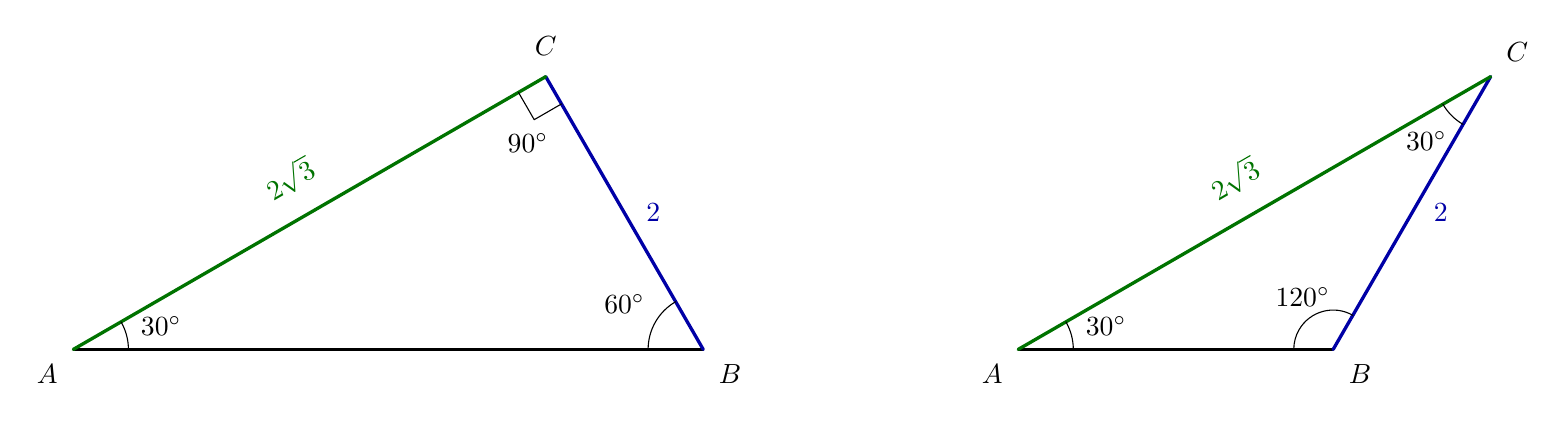
\begin{tikzpicture}[scale=2, line join=round, line cap=round]
\pgfmathsetmacro{\height}{sqrt(3)}
\def\offset{6}
\colorlet{sideblue}{blue!65!black}
\colorlet{sidegreen}{green!45!black}

\coordinate (Al) at (0,0);
\coordinate (Bl) at (4,0);
\coordinate (Cl) at (3,\height);
\coordinate (Ar) at (\offset,0);
\coordinate (Br) at ($(Ar)+(2,0)$);
\coordinate (Cr) at ($(Ar)+(3,\height)$);

\draw[thick, black] (Al) -- (Bl);
\draw[very thick, sideblue] (Bl) -- (Cl)
    node[midway, right=4pt, text=sideblue] {$2$};
\draw[very thick, sidegreen] (Al) -- (Cl)
    node[midway, sloped, above=5pt, text=sidegreen] {$2\sqrt3$};

\draw[thick, black] (Ar) -- (Br);
\draw[very thick, sideblue] (Br) -- (Cr)
    node[midway, right=4pt, text=sideblue] {$2$};
\draw[very thick, sidegreen] (Ar) -- (Cr)
    node[midway, sloped, above=5pt, text=sidegreen] {$2\sqrt3$};

\pic["$30^\circ$", draw=black, angle radius=7mm, angle eccentricity=1.65]
    {angle=Bl--Al--Cl};
\pic["$60^\circ$", draw=black, angle radius=7mm, angle eccentricity=1.65]
    {angle=Cl--Bl--Al};
\pic["$90^\circ$", draw=black, angle radius=4mm, angle eccentricity=1.55]
    {right angle=Al--Cl--Bl};

\pic["$30^\circ$", draw=black, angle radius=7mm, angle eccentricity=1.65]
    {angle=Br--Ar--Cr};
\pic["$120^\circ$", draw=black, angle radius=5mm, angle eccentricity=1.55]
    {angle=Cr--Br--Ar};
\pic["$30^\circ$", draw=black, angle radius=7mm, angle eccentricity=1.65]
    {angle=Ar--Cr--Br};

\node[below left=3pt] at (Al) {$A$};
\node[below right=3pt] at (Bl) {$B$};
\node[above=4pt] at (Cl) {$C$};
\node[below left=3pt] at (Ar) {$A$};
\node[below right=3pt] at (Br) {$B$};
\node[above right=3pt] at (Cr) {$C$};
\end{tikzpicture}
% end q000726 figure F1
\end{djsSolutionFigure}

For two sides of lengths $a$ and $b$ enclosing an angle $C$, the area is $\frac12ab\sin C$. Here the given sides $BC$ and $AC$ enclose $\angle ACB$, so the two areas are
\[
\begin{aligned}
\frac12(2)(2\sqrt3)\sin90^\circ&=2\sqrt3\\[5pt]
\frac12(2)(2\sqrt3)\sin30^\circ&=\sqrt3
\end{aligned}
\]

Their sum is
\[
2\sqrt3+\sqrt3=\boxed{3\sqrt3}
\]

The correct option is \textbf{C}.\\[5pt]

\textit{Alternative Solution:}

The cosine rule gives a quadratic whose roots are the two possible lengths $AB$. We need only their sum, because the area is proportional to $AB$.

Write $AB=x$. The cosine rule gives
\[
BC^2=AC^2+AB^2-2(AC)(AB)\cos\angle BAC
\]

Substituting,
\[
2^2=(2\sqrt3)^2+x^2-2(2\sqrt3)x\cos30^\circ
\implies 4=12+x^2-6x
\implies x^2-6x+8=0
\]

For a quadratic $ax^2+bx+c=0$, the sum of the roots is $-b/a$. The sum of the two possible lengths $AB$ is therefore
\[
-\frac{-6}{1}=6
\]

Using the sides meeting at $A$, the area of either triangle is
\[
\frac12(AC)(AB)\sin\angle BAC
=\frac12(2\sqrt3)x\sin30^\circ
=\frac{\sqrt3}{2}x
\]

Hence the sum of the areas is
\[
\frac{\sqrt3}{2}\times6=3\sqrt3
\]

Again, the correct option is \textbf{C}.
% end q000726 solution
\end{djsSolution}
\end{enumerate}
\clearpage
\thispagestyle{djssolutions}
\vspace*{8pt}
\djsTopicLine{Logic}
\begin{enumerate}[label=\textbf{\arabic*.},leftmargin=*,itemsep=0pt,start=2]
\questionitem[Logic]
% begin q000121 stem
Let $f(x),\, g(x)$ and $h(x)$ be real functions and consider the statement \begin{equation}\tag{$\ast$} \text{If $x>0$ and $f(x)\le 0$ then $g(x)\neq 1$ or $h(x)\ge -1$}\\[5pt] \end{equation} Which of the following statements is the \textit{contrapositive} of ($\ast$)?
% end q000121 stem

\par\vspace*{12pt}
\begin{tabularx}{\linewidth}{@{}>{\bfseries}l Y@{}}
A &
% begin q000121 choice A
If $g(x) = 1$ and $h(x) < -1$ then $x \le 0$ or $f(x) > 0$
% end q000121 choice A
\\[0.8em]
B &
% begin q000121 choice B
If $g(x) = 1$ or $h(x) < -1$ then $x \le 0$ or $f(x) > 0$
% end q000121 choice B
\\[0.8em]
C &
% begin q000121 choice C
If $x \le 0$ or $f(x) > 0$ then $g(x) = 1$ and $h(x) < -1$
% end q000121 choice C
\\[0.8em]
D &
% begin q000121 choice D
If $g(x) \neq 1$ or $h(x) \ge -1$ then $x > 0$ and $f(x) \le 0$
% end q000121 choice D
\\[0.8em]
E &
% begin q000121 choice E
If $x > 0$ and $f(x) \le 0$ then $g(x) = 1$ and $h(x) < -1$
% end q000121 choice E
\\[0.8em]
F &
% begin q000121 choice F
If $g(x) = 1$ and $h(x) < -1$ then $x \le 0$ and $f(x) > 0$
% end q000121 choice F
\\
\end{tabularx}

\begin{djsSolution}{A}
% begin q000121 solution
The contrapositive of a statement of the form
\[
\text{if P, then Q}
\]
is the statement
\[
\text{if not Q, then not P}
\]

The contrapositive is equivalent to the original statement: if P always leads to Q, then whenever Q fails, P cannot hold.

To form it, we negate P and Q and swap their order. For ($\ast$),
\[
\begin{array}{@{}ll@{}}
\text{P:} & x>0\text{ and }f(x)\le0\\[5pt]
\text{Q:} & g(x)\neq1\text{ or }h(x)\ge-1
\end{array}
\]

Each of P and Q joins two simple conditions with ``and'' or ``or''. Negating such a statement negates each simple condition and changes
\[
\text{``and''}\quad\longleftrightarrow\quad\text{``or''}
\]

An ``and'' statement is false when at least one of its conditions is false, so its negation uses ``or''. An ``or'' statement is false only when both of its conditions are false, so its negation uses ``and''.

Now negate the four simple conditions one at a time:
\[
\begin{array}{rcl}
x>0 &\longrightarrow& x\le0\\[5pt]
f(x)\le0 &\longrightarrow& f(x)>0\\[5pt]
g(x)\neq1 &\longrightarrow& g(x)=1\\[5pt]
h(x)\ge-1 &\longrightarrow& h(x)<-1
\end{array}
\]

Take care with equality: negating a strict inequality gives a non-strict one, and negating a non-strict inequality gives a strict one. For example, $x=0$ makes $x>0$ false, so it belongs in $x\le0$, while $h(x)=-1$ makes $h(x)\ge-1$ true, so it is excluded from $h(x)<-1$.

Applying the ``and''/``or'' rule to these gives
\[
\begin{array}{@{}ll@{}}
\text{not P:} & x\le0\text{ or }f(x)>0\\[5pt]
\text{not Q:} & g(x)=1\text{ and }h(x)<-1
\end{array}
\]

Keeping ``and'' when negating P would give option F, and keeping ``or'' when negating Q would give option B.

Finally, place the negations in the order ``if not Q, then not P''. Leaving them in the original order would give ``if not P, then not Q'', which is option C and is not equivalent to ($\ast$).

The contrapositive of ($\ast$) is therefore
\[
\boxed{\text{If }g(x)=1\text{ and }h(x)<-1\text{ then }x\le0\text{ or }f(x)>0}
\]

The correct option is \textbf{A}.
% end q000121 solution
\end{djsSolution}
\end{enumerate}
\clearpage
\thispagestyle{djssolutions}
\vspace*{8pt}
\djsTopicLine{Logic}
\begin{enumerate}[label=\textbf{\arabic*.},leftmargin=*,itemsep=0pt,start=3]
\questionitem[Logic]
% begin q000723 stem
Consider the equation

\[
4^x - 3 \times 2^x + k = 0
\]

where $k$ is a real constant.

Which of the following statements is/are true?

\[
\begin{array}{@{}ll@{}}
\textbf{I} & \text{For the equation to have a real solution, it is necessary that } k < 0 \\[5pt]
\textbf{II} & \text{For the equation to have a real solution, it is sufficient that } k < 0 \\[5pt]
\textbf{III} & \text{For the equation to have two distinct real solutions, it is necessary and} \\
& \text{sufficient that } 0 < k < \dfrac{9}{4} \\[5pt]
\end{array}
\]
% end q000723 stem

\par\vspace*{12pt}
\begin{tabularx}{\linewidth}{@{}>{\bfseries}l Y@{}}
A &
% begin q000723 choice A
None of them
% end q000723 choice A
\\[0.8em]
B &
% begin q000723 choice B
I only
% end q000723 choice B
\\[0.8em]
C &
% begin q000723 choice C
II only
% end q000723 choice C
\\[0.8em]
D &
% begin q000723 choice D
III only
% end q000723 choice D
\\[0.8em]
E &
% begin q000723 choice E
I and II only
% end q000723 choice E
\\[0.8em]
F &
% begin q000723 choice F
I and III only
% end q000723 choice F
\\[0.8em]
G &
% begin q000723 choice G
II and III only
% end q000723 choice G
\\[0.8em]
H &
% begin q000723 choice H
I, II and III
% end q000723 choice H
\\
\end{tabularx}

\begin{djsSolution}{G}
% begin q000723 solution
Statement I says that $k<0$ is necessary for a real solution: the equation cannot have a real solution unless $k<0$. That is, if the equation has a real solution, then $k<0$.

Statement II says that $k<0$ is sufficient for a real solution: $k<0$ on its own guarantees one. That is, if $k<0$, then the equation has a real solution.

Statement III says that $0<k<\frac94$ is both necessary and sufficient for two distinct real solutions. That is, if the equation has two distinct real solutions, then $0<k<\frac94$; and if $0<k<\frac94$, then the equation has two distinct real solutions.

Put $t=2^x$ to turn the exponential equation into a quadratic. Since $4^x=(2^x)^2$, we obtain
\[
t^2-3t+k=0,\qquad t>0
\]

The function $2^x$ is strictly increasing and takes every positive value, so each positive root $t$ gives exactly one real solution $x=\log_2 t$. Zero and negative roots give no real solution of the original equation.

To disprove I, we need a value $k\geq0$ for which the equation has a real solution.

Take $k=2$. The numbers $1$ and $2$ have sum $3$ and product $2$, so
\[
t^2-3t+2=(t-1)(t-2)=0
\implies t=1\text{ or }t=2
\]

These positive roots give $x=0$ or $x=1$, despite $k=2>0$. Statement I is false.

To prove II, we must show that every negative value of $k$ gives a positive root $t$. When $k<0$, the quadratic has positive discriminant:
\[
9-4k>9>0
\]

It therefore has two distinct real roots, which we call $\alpha$ and $\beta$. For a quadratic $at^2+bt+c=0$, the sum of the roots is $-b/a$ and their product is $c/a$, so here
\[
\alpha+\beta=-\frac{-3}{1}=3
\qquad\text{and}\qquad
\alpha\beta=\frac{k}{1}=k<0
\]

The negative product means that one root is positive and the other is negative. The positive root gives a real solution $x$, so II is true.

For III, first check necessity. Two distinct real solutions $x$ require two distinct positive roots $t$, so the discriminant and the product of the roots must both be positive:
\[
9-4k>0\quad\text{and}\quad k>0
\implies 0<k<\frac94
\]

Now check sufficiency. If $0<k<\frac94$, the discriminant is positive, so there are two distinct real roots, and their product $k$ is positive, so both roots have the same sign.

Their sum is $3>0$, so both roots must be positive. They therefore give two distinct real solutions $x$.

The condition for exactly two distinct real solutions is consequently
\[
\boxed{0<k<\frac94}
\]

Statements II and III are true, so the correct option is \textbf{G}.\\[5pt]

\textit{Alternative Solution:}

Using the same substitution $t=2^x>0$, rearrange the equation as
\[
k=3t-t^2
\]

Positive roots $t$ are the intersections of the curve $y=3t-t^2$, restricted to $t>0$, with the horizontal line $y=k$. Completing the square gives
\[
y=3t-t^2=\frac94-\left(t-\frac32\right)^2
\]

The vertex is $\left(\frac32,\frac94\right)$, and the curve meets the horizontal axis at $t=3$; the origin is excluded because $t>0$.

\begin{djsSolutionFigure}
% begin q000723 figure F1
\begin{tikzpicture}[x=2.6cm,y=1.15cm]
\def\tmin{-0.3}
\def\tmax{4.25}
\def\ymin{-3.1}
\def\ymax{3.85}
\def\yend{-3}
\def\kneg{-1.5}
\def\kmid{1}
\def\khigh{3.25}
\pgfmathsetmacro{\tv}{3/2}
\pgfmathsetmacro{\yv}{9/4}
\pgfmathsetmacro{\tend}{(3+sqrt(9-4*(\yend)))/2}
\pgfmathsetmacro{\tneg}{(3+sqrt(9-4*(\kneg)))/2}
\pgfmathsetmacro{\tmidL}{(3-sqrt(9-4*(\kmid)))/2}
\pgfmathsetmacro{\tmidR}{(3+sqrt(9-4*(\kmid)))/2}
\coordinate (O) at (0,0);
\coordinate (V) at (\tv,\yv);
\coordinate (R) at (3,0);
\coordinate (Pneg) at (\tneg,\kneg);
\coordinate (PmidL) at (\tmidL,\kmid);
\coordinate (PmidR) at (\tmidR,\kmid);

\foreach \level in {\kneg,\kmid,\yv,\khigh}{\draw[thin,dashed,black!45] (0,\level) -- (\tmax,\level);}

\draw[thin,black,-{Stealth[length=2.2mm]}] (\tmin,0) -- (\tmax,0)
  node[below=2pt] {$t$};
\draw[thin,black,-{Stealth[length=2.2mm]}] (0,\ymin) -- (0,\ymax)
  node[left=2pt] {$y$};

\draw[blue!65!black,line width=1.3pt]
  plot[domain=0:\tend,samples=120,smooth,variable=\t]
  (\t,{3*(\t)-(\t)^2});

\fill[red!70!black] (Pneg) circle[radius=2.4pt];
\fill[red!70!black] (R) circle[radius=2.4pt];
\fill[red!70!black] (PmidL) circle[radius=2.4pt];
\fill[red!70!black] (PmidR) circle[radius=2.4pt];
\fill[red!70!black] (V) circle[radius=2.4pt];
\draw[blue!65!black,line width=1pt,fill=white] (O) circle[radius=2.4pt];

\node[below left=2pt] at (O) {$0$};
\node[below left=2pt] at (R) {$3$};
\node[above=4pt] at (V) {$\left(\frac{3}{2},\frac{9}{4}\right)$};

\node[right=6pt] at (\tmax,\kneg) {$k<0$};
\node[right=6pt] at (\tmax,0) {$k=0$};
\node[right=6pt] at (\tmax,\kmid) {$0<k<\frac{9}{4}$};
\node[right=6pt] at (\tmax,\yv) {$k=\frac{9}{4}$};
\node[right=6pt] at (\tmax,\khigh) {$k>\frac{9}{4}$};
\end{tikzpicture}
% end q000723 figure F1
\end{djsSolutionFigure}

The sketch shows the number of intersections at each horizontal level:
\[
\begin{array}{c|c}
\text{Value of }k & \text{Number of positive roots }t\\[5pt]
\hline
k<0 & 1\\[5pt]
k=0 & 1\\[5pt]
0<k<\frac94 & 2\\[8pt]
k=\frac94 & 1\\[8pt]
k>\frac94 & 0
\end{array}
\]

At $k=0$, the only allowed root is $t=3$: the root $t=0$ is excluded. At the maximum level $k=\frac94$, the line touches the curve at $t=\frac32$, giving only one distinct root.

Each positive root gives exactly one real solution $x$. Thus $k<0$ guarantees a real solution but is not required, and exactly two distinct real solutions occur when $0<k<\frac94$.

Again, II and III are true, giving option \textbf{G}.
% end q000723 solution
\end{djsSolution}
\end{enumerate}
\clearpage
\thispagestyle{djssolutions}
\vspace*{8pt}
\djsTopicLine{Logic}
\begin{enumerate}[label=\textbf{\arabic*.},leftmargin=*,itemsep=0pt,start=4]
\questionitem[Logic]
% begin q000724 stem
An infinite geometric series
\[
a + ar + ar^2 + ar^3 + \cdots
\]
where $a \ne 0$, has sum to infinity $S$.

Which of the following statements is/are true?
\[
\begin{array}{@{}ll@{}}
\textbf{I} & S > a \textbf{ only if } r > 0 \\[5pt]
\textbf{II} & r > 0 \text{ is }\textbf{sufficient}\text{ for } S>a  \\[5pt]
\textbf{III} & a \text{ and } r \text{ being both positive or both negative is}\textbf{ necessary and sufficient} \text{ for } S > a
\end{array}
\]
% end q000724 stem

\par\vspace*{12pt}
\begin{tabularx}{\linewidth}{@{}>{\bfseries}l Y@{}}
A &
% begin q000724 choice A
None of them
% end q000724 choice A
\\[0.8em]
B &
% begin q000724 choice B
I only
% end q000724 choice B
\\[0.8em]
C &
% begin q000724 choice C
II only
% end q000724 choice C
\\[0.8em]
D &
% begin q000724 choice D
III only
% end q000724 choice D
\\[0.8em]
E &
% begin q000724 choice E
I and II only
% end q000724 choice E
\\[0.8em]
F &
% begin q000724 choice F
I and III only
% end q000724 choice F
\\[0.8em]
G &
% begin q000724 choice G
II and III only
% end q000724 choice G
\\[0.8em]
H &
% begin q000724 choice H
I, II and III
% end q000724 choice H
\\
\end{tabularx}

\begin{djsSolution}{D}
% begin q000724 solution
Since the series has a sum to infinity and $a\ne0$, we have $|r|<1$. The sum-to-infinity formula is
\[
S=\frac{a}{1-r}
\]

In particular, $1-r>0$, so multiplying an inequality by $1-r$ preserves its direction:
\[
S>a
\iff \frac{a}{1-r}>a
\iff a>a(1-r)
\iff \boxed{ar>0}
\]

A product is positive exactly when both factors are positive or both are negative. If $r=0$, then $S=a$, so the strict inequality does not hold.

Statement I says: if $S>a$, then $r>0$. To disprove it, we need an allowed series with $S>a$ but $r\leq0$; take $a=-1$ and $r=-\frac12$:
\[
S=\frac{-1}{1-(-\frac12)}=-\frac23>-1=a
\]

Here $S>a$ but $r<0$, so I is false.

Statement II says: if $r>0$, then $S>a$. To disprove it, take $a=-1$ and $r=\frac12$:
\[
S=\frac{-1}{1-\frac12}=-2<-1=a
\]

Here $r>0$ but $S>a$ is false, so II is false.

Now check both directions of III. The necessary direction says: if $S>a$, then $a$ and $r$ are both positive or both negative.

We have shown that $S>a$ requires $ar>0$, which requires both factors to be positive or both to be negative. Thus the condition is necessary.

The sufficient direction says: if $a$ and $r$ are both positive or both negative, then $S>a$. In either case $ar>0$, and the reversible calculation above gives $S>a$, so the condition is sufficient.

This also explains why III is incompatible with I and II: the both-negative case contradicts I, while III rules out $S>a$ when $a<0<r$, contrary to II.

Only III is true, so the correct option is \textbf{D}.
% end q000724 solution
\end{djsSolution}
\end{enumerate}
\clearpage
\thispagestyle{djssolutions}
\vspace*{8pt}
\djsTopicLine{Proof \& Error Analysis}
\begin{enumerate}[label=\textbf{\arabic*.},leftmargin=*,itemsep=0pt,start=5]
\questionitem[Proof \& Error Analysis]
% begin q000617 stem
A student proves that $\sqrt{2}$ is irrational, using proof by contradiction. The proof uses the following five statements, presented here in a scrambled order. \\

\begin{tabular}{@{}r@{\hspace{0.6em}}p{\dimexpr\linewidth-2.6em\relax}@{}}
(1) &
Since $p$ is even, write $p = 2k$ for some positive integer $k$; substituting into $p^2 = 2q^2$ gives $4k^2 = 2q^2$, so $q^2 = 2k^2$, and therefore $q$ is even.
\\[0.8em]

(2) &
Suppose, for contradiction, that $\sqrt{2}$ is rational, so $\sqrt{2} = \dfrac{p}{q}$ for some positive integers $p$ and $q$ with no common factor greater than $1$.
\\[0.8em]

(3) &
This means $p$ and $q$ share the common factor $2$, contradicting the assumption that $p$ and $q$ have no common factor greater than $1$.
\\[0.8em]

(4) &
Squaring both sides of $\sqrt{2} = \dfrac{p}{q}$ gives $p^2 = 2q^2$, so $p^2$ is even, and therefore $p$ is even.
\\[0.8em]

(5) &
Therefore the original assumption is false, and $\sqrt{2}$ is irrational.\\[0.8em]
\end{tabular}

\medskip

Which ordering of the statements (1)--(5) gives a valid proof, with each statement following logically from those before it?
% end q000617 stem

\par\vspace*{12pt}
\begin{tabularx}{\linewidth}{@{}>{\bfseries}l Y@{}}
A &
% begin q000617 choice A
2, 4, 1, 3, 5
% end q000617 choice A
\\[0.8em]
B &
% begin q000617 choice B
2, 1, 4, 3, 5
% end q000617 choice B
\\[0.8em]
C &
% begin q000617 choice C
4, 2, 1, 3, 5
% end q000617 choice C
\\[0.8em]
D &
% begin q000617 choice D
2, 4, 3, 1, 5
% end q000617 choice D
\\[0.8em]
E &
% begin q000617 choice E
2, 4, 1, 5, 3
% end q000617 choice E
\\[0.8em]
F &
% begin q000617 choice F
2, 3, 4, 1, 5
% end q000617 choice F
\\[0.8em]
G &
% begin q000617 choice G
2, 4, 3, 5, 1
% end q000617 choice G
\\[0.8em]
H &
% begin q000617 choice H
No ordering of the statements gives a valid proof.
% end q000617 choice H
\\
\end{tabularx}

\begin{djsSolution}{A}
% begin q000617 solution
A proof by contradiction starts by assuming the opposite of what we want to prove. Statement $(2)$ therefore comes first: it assumes that $\sqrt{2}$ is rational and writes it as $p/q$, where $p$ and $q$ have no common factor greater than $1$.

Statement $(4)$ uses this fraction to show that $p$ is even:
\[
2=\frac{p^2}{q^2}\implies p^2=2q^2
\]

Since $p^2$ is even, $p$ is even.

Statement $(1)$ needs this fact before it can write $p=2k$. Substituting gives
\[
(2k)^2=2q^2\implies 4k^2=2q^2\implies q^2=2k^2
\]

Thus $q^2$ is even, so $q$ is also even.

Statement $(3)$ can now identify the contradiction: both $p$ and $q$ are even, so they share the factor $2$, contrary to the assumption in statement $(2)$. It must follow statement $(1)$, because both integers must have been shown to be even.

Finally, statement $(5)$ rejects the original assumption and concludes that $\sqrt{2}$ is irrational. The required order is
\[
\boxed{2,\ 4,\ 1,\ 3,\ 5}
\]

The correct option is \textbf{A}.\\[5pt]

\textit{Remark:}

The contrapositive of ``if $A$, then $B$'' is ``if not $B$, then not $A$''. A statement and its contrapositive are logically equivalent.

To justify ``if an integer's square is even, then the integer is even'', prove its contrapositive: if an integer is odd, then its square is odd. An odd integer can be written as $2n+1$, where $n$ is an integer, and
\[
(2n+1)^2=4n^2+4n+1=2(2n^2+2n)+1
\]

This is odd because it is one more than an even integer. The contrapositive therefore justifies the even-square steps in statements $(4)$ and $(1)$.
% end q000617 solution
\end{djsSolution}
\end{enumerate}
\clearpage
\thispagestyle{djssolutions}
\vspace*{8pt}
\djsTopicLine{Sequences \& Series}
\begin{enumerate}[label=\textbf{\arabic*.},leftmargin=*,itemsep=0pt,start=6]
\questionitem[Sequences \& Series]
% begin q000768 stem
A geometric progression has a real first term and a real common ratio.

The sum of the first three terms is $14$, and the sum of the first six terms is $126$.

What is the sum of the first nine terms?
% end q000768 stem

\par\vspace*{12pt}
\begin{tabularx}{\linewidth}{@{}>{\bfseries}l Y@{}}
A &
% begin q000768 choice A
$98$
% end q000768 choice A
\\[0.8em]
B &
% begin q000768 choice B
$252$
% end q000768 choice B
\\[0.8em]
C &
% begin q000768 choice C
$511$
% end q000768 choice C
\\[0.8em]
D &
% begin q000768 choice D
$1022$
% end q000768 choice D
\\[0.8em]
E &
% begin q000768 choice E
$1092$
% end q000768 choice E
\\[0.8em]
F &
% begin q000768 choice F
$1134$
% end q000768 choice F
\\
\end{tabularx}

\begin{djsSolution}{D}
% begin q000768 solution
The question gives the sums of the first three and the first six terms, and asks for the sum of the first nine. Since these are all multiples of three, it helps to split the progression into blocks of three consecutive terms.

Write $a$ for the first term and $r$ for the common ratio. The first nine terms are
\[
a,\quad ar,\quad ar^2,\quad ar^3,\quad ar^4,\quad ar^5,\quad ar^6,\quad ar^7,\quad ar^8
\]

Grouping them into three blocks, the sum of the first nine terms is
\[
\underbrace{a+ar+ar^2}_{\text{first block}}
+\underbrace{ar^3+ar^4+ar^5}_{\text{second block}}
+\underbrace{ar^6+ar^7+ar^8}_{\text{third block}}
\]

Each term in the second and third blocks is $r^3$ times the term three places earlier, which lies in the block before. For example, $ar^4=r^3\times ar$ and $ar^7=r^3\times ar^4$.

Taking out the common factor $r^3$ from the second and third blocks therefore gives
\[
\begin{aligned}
ar^3+ar^4+ar^5&=r^3\left(a+ar+ar^2\right)\\[5pt]
ar^6+ar^7+ar^8&=r^3\left(ar^3+ar^4+ar^5\right)
\end{aligned}
\]

So the sum of each block is $r^3$ times the sum of the block before it.

The first block is the first three terms, so its sum is $14$. The second block is the first six terms with the first three removed, so its sum is
\[
126-14=112
\]

Since the second block sum is $r^3$ times the first,
\[
112=14r^3 \implies r^3=\frac{112}{14}=8
\]

The third block, containing terms seven to nine, therefore has sum
\[
8\times112=896
\]

Adding this to the sum of the first six terms gives
\[
126+896=\boxed{1022}
\]

There is no need to find the first term or the common ratio separately. The correct option is \textbf{D}.\\[5pt]

\textit{Alternative Solution:}

If $r=1$, all terms are equal, so the sum of the first six terms would be $2\times14=28$, not $126$. Thus $r\ne1$.

Write the first term as $a$. For $r\ne1$, the finite geometric series formula is
\[
S_n=\frac{a(r^n-1)}{r-1}
\]

Applying it to the two given sums gives
\[
\frac{a(r^3-1)}{r-1}=14
\qquad\text{and}\qquad
\frac{a(r^6-1)}{r-1}=126
\]

Dividing the second equation by the first gives
\[
\frac{r^6-1}{r^3-1}=\frac{126}{14}=9
\]

Since $r$ is real and $r\ne1$, we have $r^3-1\ne0$. Factorising $r^6-1=(r^3-1)(r^3+1)$ and cancelling gives
\[
\frac{(r^3-1)(r^3+1)}{r^3-1}=9
\implies r^3+1=9
\implies r^3=8
\implies r=2
\]

Now the three-term sum determines $a$:
\[
\frac{a(2^3-1)}{2-1}=14
\implies 7a=14
\implies a=2
\]

The sum of the first nine terms is therefore
\[
S_9=\frac{2(2^9-1)}{2-1}=2(512-1)=1022
\]

Again, the correct option is \textbf{D}.
% end q000768 solution
\end{djsSolution}
\end{enumerate}
\clearpage
\thispagestyle{djssolutions}
\vspace*{8pt}
\djsTopicLine{Logic}
\begin{enumerate}[label=\textbf{\arabic*.},leftmargin=*,itemsep=0pt,start=7]
\questionitem[Logic]
% begin q000685 stem
Let $\theta$ be a real number with $0 < \theta < 2\pi$.

Consider the following three statements about the inequality \(\sin\theta + \cos\theta > 1\)

\[
\begin{array}{@{}l l@{}}
\textbf{I:} & \text{A necessary condition for the inequality to hold is that $\sin\theta\cos\theta > 0$} \\[5pt]
\textbf{II:} & \text{A sufficient condition for the inequality to hold is that $\sin\theta\cos\theta > 0$} \\[5pt]
\textbf{III:} &
\begin{aligned}[t]
&\text{A necessary and sufficient condition for the inequality to hold is that} \\
&\sin\theta\cos\theta > 0 \text{ and } \sin\theta + \cos\theta > 0 
\end{aligned}
\end{array}
\]

Which of the statements is/are true?
% end q000685 stem

\par\vspace*{12pt}
\begin{tabularx}{\linewidth}{@{}>{\bfseries}l Y@{}}
A &
% begin q000685 choice A
None of them
% end q000685 choice A
\\[0.8em]
B &
% begin q000685 choice B
I only
% end q000685 choice B
\\[0.8em]
C &
% begin q000685 choice C
II only
% end q000685 choice C
\\[0.8em]
D &
% begin q000685 choice D
III only
% end q000685 choice D
\\[0.8em]
E &
% begin q000685 choice E
I and II only
% end q000685 choice E
\\[0.8em]
F &
% begin q000685 choice F
I and III only
% end q000685 choice F
\\[0.8em]
G &
% begin q000685 choice G
II and III only
% end q000685 choice G
\\[0.8em]
H &
% begin q000685 choice H
I, II and III
% end q000685 choice H
\\
\end{tabularx}

\begin{djsSolution}{F}
% begin q000685 solution
A condition is necessary if the inequality cannot hold without it. A condition is sufficient if it guarantees that the inequality holds.

A condition is necessary and sufficient if both directions hold.

Using $\sin^2\theta+\cos^2\theta=1$, we have
\[
\begin{aligned}
(\sin\theta+\cos\theta)^2
&=\sin^2\theta+2\sin\theta\cos\theta+\cos^2\theta\\[5pt]
&=1+2\sin\theta\cos\theta
\end{aligned}
\]

Statement I says: if $\sin\theta+\cos\theta>1$, then $\sin\theta\cos\theta>0$. Since the sum is greater than $1$, it is positive, so squaring preserves the inequality:
\[
(\sin\theta+\cos\theta)^2>1
\implies 1+2\sin\theta\cos\theta>1
\implies \sin\theta\cos\theta>0
\]

Thus I is true.

Statement II says: if $\sin\theta\cos\theta>0$, then $\sin\theta+\cos\theta>1$. To disprove this, we need an allowed angle for which the product is positive but the sum is not greater than $1$.

Take $\theta=\frac{5\pi}{4}$, which lies between $0$ and $2\pi$. Here $\sin\theta=\cos\theta=-\frac{\sqrt2}{2}$, so
\[
\begin{aligned}
\sin\theta\cos\theta
&=\left(-\frac{\sqrt2}{2}\right)^2=\frac12>0\\[8pt]
\sin\theta+\cos\theta
&=-\frac{\sqrt2}{2}-\frac{\sqrt2}{2}=-\sqrt2<1
\end{aligned}
\]

The proposed sufficient condition holds, but the inequality fails. Thus II is false.

For the necessity in III, we must show: if $\sin\theta+\cos\theta>1$, then $\sin\theta\cos\theta>0$ and $\sin\theta+\cos\theta>0$. Statement I gives the product condition, and a sum greater than $1$ is also positive.

For the sufficiency in III, we must show: if $\sin\theta\cos\theta>0$ and $\sin\theta+\cos\theta>0$, then $\sin\theta+\cos\theta>1$. The positive product gives
\[
(\sin\theta+\cos\theta)^2=1+2\sin\theta\cos\theta>1
\]

A real number whose square is greater than $1$ is either greater than $1$ or less than $-1$. The additional condition $\sin\theta+\cos\theta>0$ excludes the negative case, leaving
\[
\sin\theta+\cos\theta>1
\]

Both directions hold, so III is true. Therefore I and III only are true, giving option \textbf{F}.
% end q000685 solution
\end{djsSolution}
\end{enumerate}
\clearpage
\thispagestyle{djssolutions}
\vspace*{8pt}
\djsTopicLine{Geometry}
\begin{enumerate}[label=\textbf{\arabic*.},leftmargin=*,itemsep=0pt,start=8]
\questionitem[Geometry]
% begin q000649 stem
A solid cuboid has edges of length $1$ cm, $2$ cm and $3$ cm. 

An ant starts at one corner $S$ of the cuboid and crawls across the outside surfaces to the corner $F$ furthest from it. That is, the corner not sharing any face with the starting corner. 

The ant may cross any face but cannot pass through the inside of the cuboid. 

What is the shortest possible distance the ant travels?
% end q000649 stem

\begin{center}
% begin q000649 diagram
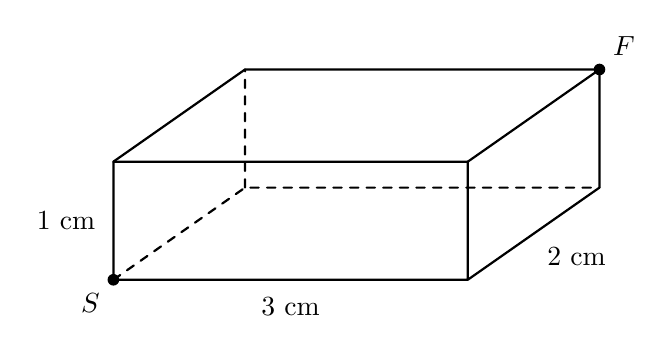
\begin{tikzpicture}[scale=1.5, line join=round, line cap=round]
\def\cuboidlength{3}
\def\cuboiddepth{2}
\def\cuboidheight{1}
\def\depthangle{35}
\pgfmathsetmacro{\projecteddepth}{0.68*\cuboiddepth}

% Projected cuboid vertices
\coordinate (S) at (0,0);
\coordinate (B) at (\cuboidlength,0);
\coordinate (D) at ($(S)+(\depthangle:\projecteddepth)$);
\coordinate (C) at ($(B)+(\depthangle:\projecteddepth)$);
\coordinate (A) at ($(S)+(0,\cuboidheight)$);
\coordinate (E) at ($(B)+(0,\cuboidheight)$);
\coordinate (H) at ($(D)+(0,\cuboidheight)$);
\coordinate (F) at ($(C)+(0,\cuboidheight)$);

% Hidden edges
\draw[thick, dashed, black] (S) -- (D) -- (C);
\draw[thick, dashed, black] (D) -- (H);

% Visible edges
\draw[thick, black] (S) -- (B) -- (E) -- (A) -- cycle;
\draw[thick, black] (B) -- (C) -- (F) -- (E);
\draw[thick, black] (A) -- (H) -- (F);

% Marked opposite corners
\fill[black] (S) circle (1.4pt);
\fill[black] (F) circle (1.4pt);

% Corner labels
\node[below left=2pt] at (S) {$S$};
\node[above right=2pt] at (F) {$F$};

% Edge-length labels
\path (S) -- (B) node[midway, below=3pt] {$3\text{ cm}$};
\path (B) -- (C) node[midway, below right=2pt] {$2\text{ cm}$};
\path (S) -- (A) node[midway, left=3pt] {$1\text{ cm}$};
\end{tikzpicture}
% end q000649 diagram
\end{center}

\par\vspace*{12pt}
\begin{tabularx}{\linewidth}{@{}>{\bfseries}l Y@{}}
A &
% begin q000649 choice A
$\sqrt{14}$ cm
% end q000649 choice A
\\[0.8em]
B &
% begin q000649 choice B
$3\sqrt{2}$ cm
% end q000649 choice B
\\[0.8em]
C &
% begin q000649 choice C
$2\sqrt{5}$ cm
% end q000649 choice C
\\[0.8em]
D &
% begin q000649 choice D
$1+\sqrt{13}$ cm
% end q000649 choice D
\\[0.8em]
E &
% begin q000649 choice E
$\sqrt{26}$ cm
% end q000649 choice E
\\[0.8em]
F &
% begin q000649 choice F
$6$ cm
% end q000649 choice F
\\
\end{tabularx}

\begin{djsSolution}{B}
% begin q000649 solution
Unfolding two faces preserves distances, and their shortest route becomes the diagonal of a rectangle. There are three different rectangle sizes, according to the length of the shared edge.

For faces sharing a $3\text{ cm}$ edge, such as the front and top faces, the unfolded rectangle has dimensions $3\text{ cm}$ by $(1+2)\text{ cm}$. In each figure below, the shared edge is orange and the route is blue.

\begin{djsSolutionFigure}
% begin q000649 figure F1
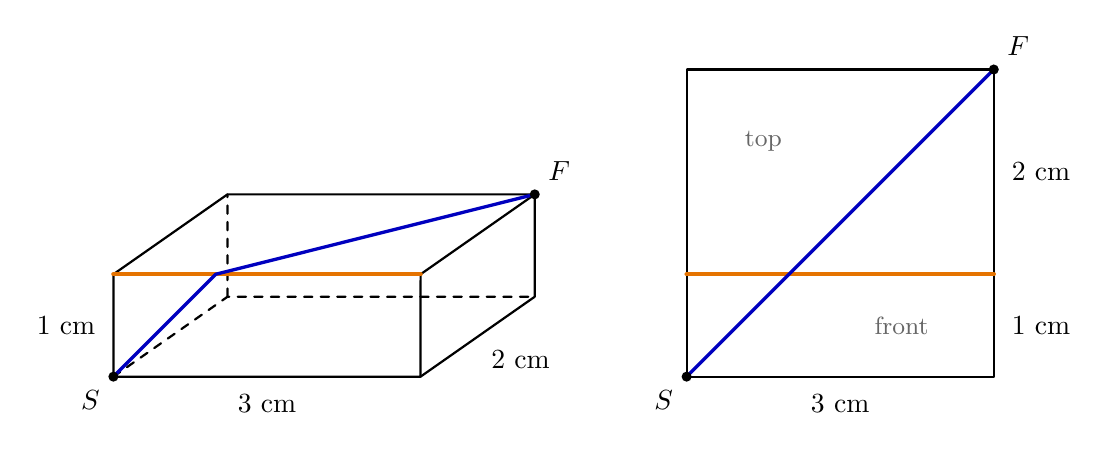
\begin{tikzpicture}[scale=1.3, line join=round, line cap=round]
\def\cuboidlength{3}
\def\cuboiddepth{2}
\def\cuboidheight{1}
\def\depthangle{35}
\def\netshift{5.6}
\pgfmathsetmacro{\projecteddepth}{0.68*\cuboiddepth}
\pgfmathsetmacro{\crossfraction}{\cuboidheight/(\cuboidheight+\cuboiddepth)}
\pgfmathsetmacro{\netheight}{\cuboidheight+\cuboiddepth}

% Cuboid vertices, as in the question
\coordinate (S) at (0,0);
\coordinate (B) at (\cuboidlength,0);
\coordinate (D) at ($(S)+(\depthangle:\projecteddepth)$);
\coordinate (C) at ($(B)+(\depthangle:\projecteddepth)$);
\coordinate (A) at ($(S)+(0,\cuboidheight)$);
\coordinate (E) at ($(B)+(0,\cuboidheight)$);
\coordinate (H) at ($(D)+(0,\cuboidheight)$);
\coordinate (F) at ($(C)+(0,\cuboidheight)$);

% Hidden edges
\draw[thick, dashed, black] (S) -- (D) -- (C);
\draw[thick, dashed, black] (D) -- (H);

% Visible edges
\draw[thick, black] (S) -- (B) -- (E) -- (A) -- cycle;
\draw[thick, black] (B) -- (C) -- (F) -- (E);
\draw[thick, black] (A) -- (H) -- (F);

% Shared 3 cm edge between the front and top faces
\draw[line width=1.6pt, orange!90!black] (A) -- (E);

% Route across the front face, then the top face
\coordinate (P) at ($(A)!\crossfraction!(E)$);
\draw[very thick, blue!75!black] (S) -- (P) -- (F);

% Marked opposite corners
\fill[black] (S) circle (1.4pt);
\fill[black] (F) circle (1.4pt);
\node[below left=2pt] at (S) {$S$};
\node[above right=2pt] at (F) {$F$};

% Edge-length labels
\path (S) -- (B) node[midway, below=3pt] {$3\text{ cm}$};
\path (B) -- (C) node[midway, below right=2pt] {$2\text{ cm}$};
\path (S) -- (A) node[midway, left=3pt] {$1\text{ cm}$};

% The front and top faces unfolded into one rectangle
\begin{scope}[shift={(\netshift,0)}]
\coordinate (NS) at (0,0);
\coordinate (NB) at (\cuboidlength,0);
\coordinate (NE) at (\cuboidlength,\cuboidheight);
\coordinate (NA) at (0,\cuboidheight);
\coordinate (NF) at (\cuboidlength,\netheight);
\coordinate (NH) at (0,\netheight);
\draw[thick, black] (NS) -- (NB) -- (NF) -- (NH) -- cycle;
\draw[line width=1.6pt, orange!90!black] (NA) -- (NE);
\draw[very thick, blue!75!black] (NS) -- (NF);
\fill[black] (NS) circle (1.4pt);
\fill[black] (NF) circle (1.4pt);
\node[below left=2pt] at (NS) {$S$};
\node[above right=2pt] at (NF) {$F$};
\path (NS) -- (NB) node[midway, below=3pt] {$3\text{ cm}$};
\path (NB) -- (NE) node[midway, right=3pt] {$1\text{ cm}$};
\path (NE) -- (NF) node[midway, right=3pt] {$2\text{ cm}$};

% Face names, matching the text
\node[font=\small, text=black!60] at ($(NA)!0.5!(NB)+(0.6,0)$) {front};
\node[font=\small, text=black!60] at ($(NA)!0.5!(NF)+(-0.75,0.3)$) {top};
\end{scope}
\end{tikzpicture}
% end q000649 figure F1
\end{djsSolutionFigure}

By Pythagoras' theorem, this route has length
\[
\sqrt{3^2+(1+2)^2}=\sqrt{18}=3\sqrt{2}\text{ cm}
\]

For faces sharing a $2\text{ cm}$ edge, such as the left and top faces, the unfolded rectangle has dimensions $2\text{ cm}$ by $(1+3)\text{ cm}$. The left face is hidden, so the part of the route on it is dashed.

\begin{djsSolutionFigure}
% begin q000649 figure F2
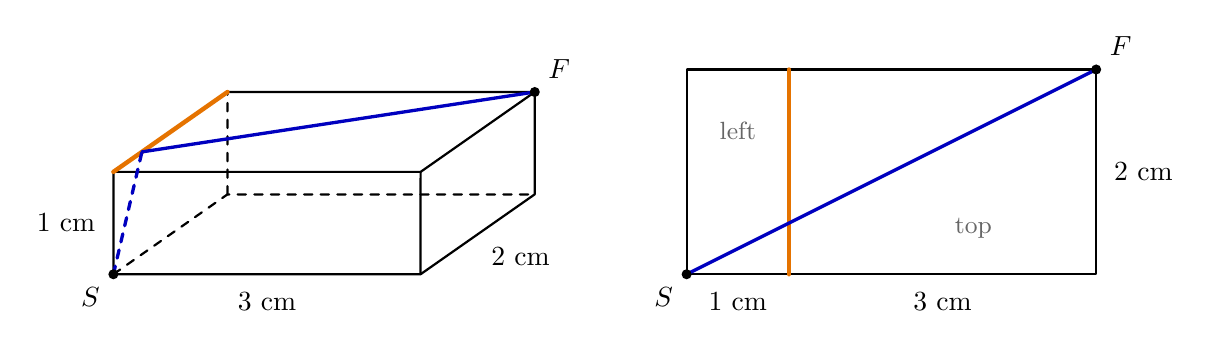
\begin{tikzpicture}[scale=1.3, line join=round, line cap=round]
\def\cuboidlength{3}
\def\cuboiddepth{2}
\def\cuboidheight{1}
\def\depthangle{35}
\def\netshift{5.6}
\pgfmathsetmacro{\projecteddepth}{0.68*\cuboiddepth}
\pgfmathsetmacro{\crossfraction}{\cuboidheight/(\cuboidheight+\cuboidlength)}
\pgfmathsetmacro{\netwidth}{\cuboidheight+\cuboidlength}

% Cuboid vertices, as in the question
\coordinate (S) at (0,0);
\coordinate (B) at (\cuboidlength,0);
\coordinate (D) at ($(S)+(\depthangle:\projecteddepth)$);
\coordinate (C) at ($(B)+(\depthangle:\projecteddepth)$);
\coordinate (A) at ($(S)+(0,\cuboidheight)$);
\coordinate (E) at ($(B)+(0,\cuboidheight)$);
\coordinate (H) at ($(D)+(0,\cuboidheight)$);
\coordinate (F) at ($(C)+(0,\cuboidheight)$);

% Hidden edges
\draw[thick, dashed, black] (S) -- (D) -- (C);
\draw[thick, dashed, black] (D) -- (H);

% Visible edges
\draw[thick, black] (S) -- (B) -- (E) -- (A) -- cycle;
\draw[thick, black] (B) -- (C) -- (F) -- (E);
\draw[thick, black] (A) -- (H) -- (F);

% Shared 2 cm edge between the left and top faces
\draw[line width=1.6pt, orange!90!black] (A) -- (H);

% Route across the hidden left face, then the top face
\coordinate (P) at ($(A)!\crossfraction!(H)$);
\draw[very thick, dashed, blue!75!black] (S) -- (P);
\draw[very thick, blue!75!black] (P) -- (F);

% Marked opposite corners
\fill[black] (S) circle (1.4pt);
\fill[black] (F) circle (1.4pt);
\node[below left=2pt] at (S) {$S$};
\node[above right=2pt] at (F) {$F$};

% Edge-length labels
\path (S) -- (B) node[midway, below=3pt] {$3\text{ cm}$};
\path (B) -- (C) node[midway, below right=2pt] {$2\text{ cm}$};
\path (S) -- (A) node[midway, left=3pt] {$1\text{ cm}$};

% The left and top faces unfolded into one rectangle
\begin{scope}[shift={(\netshift,0)}]
\coordinate (NS) at (0,0);
\coordinate (NA) at (\cuboidheight,0);
\coordinate (NE) at (\netwidth,0);
\coordinate (NF) at (\netwidth,\cuboiddepth);
\coordinate (NH) at (\cuboidheight,\cuboiddepth);
\coordinate (ND) at (0,\cuboiddepth);
\draw[thick, black] (NS) -- (NE) -- (NF) -- (ND) -- cycle;
\draw[line width=1.6pt, orange!90!black] (NA) -- (NH);
\draw[very thick, blue!75!black] (NS) -- (NF);
\fill[black] (NS) circle (1.4pt);
\fill[black] (NF) circle (1.4pt);
\node[below left=2pt] at (NS) {$S$};
\node[above right=2pt] at (NF) {$F$};
\path (NS) -- (NA) node[midway, below=3pt] {$1\text{ cm}$};
\path (NA) -- (NE) node[midway, below=3pt] {$3\text{ cm}$};
\path (NE) -- (NF) node[midway, right=3pt] {$2\text{ cm}$};

% Face names, matching the text
\node[font=\small, text=black!60] at ($(NS)!0.5!(NH)+(0,0.4)$) {left};
\node[font=\small, text=black!60] at ($(NA)!0.5!(NF)+(0.3,-0.55)$) {top};
\end{scope}
\end{tikzpicture}
% end q000649 figure F2
\end{djsSolutionFigure}

This route has length
\[
\sqrt{2^2+(1+3)^2}=\sqrt{20}=2\sqrt{5}\text{ cm}
\]

For faces sharing a $1\text{ cm}$ edge, such as the front and right faces, the unfolded rectangle has dimensions $1\text{ cm}$ by $(2+3)\text{ cm}$.

\begin{djsSolutionFigure}
% begin q000649 figure F3
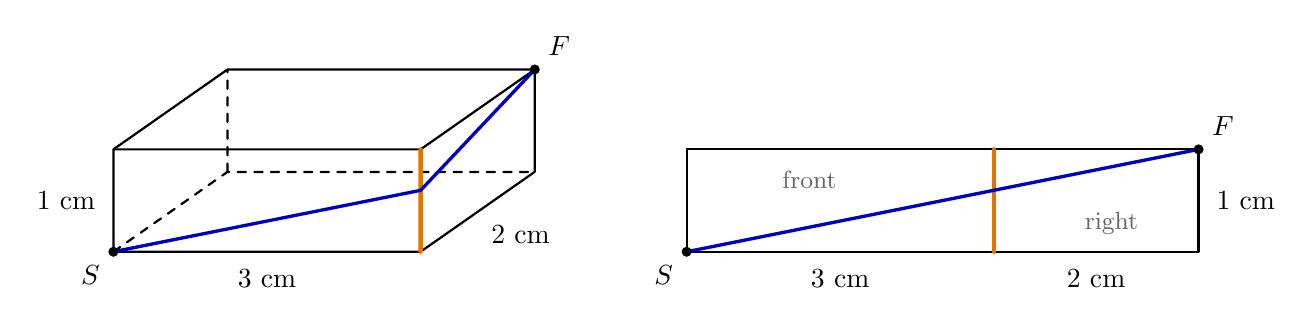
\begin{tikzpicture}[scale=1.3, line join=round, line cap=round]
\def\cuboidlength{3}
\def\cuboiddepth{2}
\def\cuboidheight{1}
\def\depthangle{35}
\def\netshift{5.6}
\pgfmathsetmacro{\projecteddepth}{0.68*\cuboiddepth}
\pgfmathsetmacro{\crossfraction}{\cuboidlength/(\cuboidlength+\cuboiddepth)}
\pgfmathsetmacro{\netwidth}{\cuboidlength+\cuboiddepth}

% Cuboid vertices, as in the question
\coordinate (S) at (0,0);
\coordinate (B) at (\cuboidlength,0);
\coordinate (D) at ($(S)+(\depthangle:\projecteddepth)$);
\coordinate (C) at ($(B)+(\depthangle:\projecteddepth)$);
\coordinate (A) at ($(S)+(0,\cuboidheight)$);
\coordinate (E) at ($(B)+(0,\cuboidheight)$);
\coordinate (H) at ($(D)+(0,\cuboidheight)$);
\coordinate (F) at ($(C)+(0,\cuboidheight)$);

% Hidden edges
\draw[thick, dashed, black] (S) -- (D) -- (C);
\draw[thick, dashed, black] (D) -- (H);

% Visible edges
\draw[thick, black] (S) -- (B) -- (E) -- (A) -- cycle;
\draw[thick, black] (B) -- (C) -- (F) -- (E);
\draw[thick, black] (A) -- (H) -- (F);

% Shared 1 cm edge between the front and right faces
\draw[line width=1.6pt, orange!90!black] (B) -- (E);

% Route across the front face, then the right face
\coordinate (P) at ($(B)!\crossfraction!(E)$);
\draw[very thick, blue!75!black] (S) -- (P) -- (F);

% Marked opposite corners
\fill[black] (S) circle (1.4pt);
\fill[black] (F) circle (1.4pt);
\node[below left=2pt] at (S) {$S$};
\node[above right=2pt] at (F) {$F$};

% Edge-length labels
\path (S) -- (B) node[midway, below=3pt] {$3\text{ cm}$};
\path (B) -- (C) node[midway, below right=2pt] {$2\text{ cm}$};
\path (S) -- (A) node[midway, left=3pt] {$1\text{ cm}$};

% The front and right faces unfolded into one rectangle
\begin{scope}[shift={(\netshift,0)}]
\coordinate (NS) at (0,0);
\coordinate (NB) at (\cuboidlength,0);
\coordinate (NC) at (\netwidth,0);
\coordinate (NF) at (\netwidth,\cuboidheight);
\coordinate (NE) at (\cuboidlength,\cuboidheight);
\coordinate (NA) at (0,\cuboidheight);
\draw[thick, black] (NS) -- (NC) -- (NF) -- (NA) -- cycle;
\draw[line width=1.6pt, orange!90!black] (NB) -- (NE);
\draw[very thick, blue!75!black] (NS) -- (NF);
\fill[black] (NS) circle (1.4pt);
\fill[black] (NF) circle (1.4pt);
\node[below left=2pt] at (NS) {$S$};
\node[above right=2pt] at (NF) {$F$};
\path (NS) -- (NB) node[midway, below=3pt] {$3\text{ cm}$};
\path (NB) -- (NC) node[midway, below=3pt] {$2\text{ cm}$};
\path (NC) -- (NF) node[midway, right=3pt] {$1\text{ cm}$};

% Face names, matching the text
\node[font=\small, text=black!60] at ($(NA)!0.5!(NB)+(-0.3,0.2)$) {front};
\node[font=\small, text=black!60] at ($(NB)!0.5!(NF)+(0.15,-0.22)$) {right};
\end{scope}
\end{tikzpicture}
% end q000649 figure F3
\end{djsSolutionFigure}

This route has length
\[
\sqrt{1^2+(2+3)^2}=\sqrt{26}\text{ cm}
\]

All three distances are positive, so we can compare their squares:
\[
18<20<26
\]

The shortest possible distance is therefore
\[
\boxed{3\sqrt{2}\text{ cm}}
\]

The correct option is \textbf{B}.
% end q000649 solution
\end{djsSolution}
\end{enumerate}
\clearpage
\thispagestyle{djssolutions}
\vspace*{8pt}
\djsTopicLine{Integration}
\begin{enumerate}[label=\textbf{\arabic*.},leftmargin=*,itemsep=0pt,start=9]
\questionitem[Integration]
% begin q000156 stem
Let $\lfloor x\rfloor$ denote the greatest integer less than or equal to $x$.

Define \[ f(x)=\lfloor 2x\rfloor-\lfloor x\rfloor \] for all real $x$.

The value of $\displaystyle \int_0^2 f(x)\,\mathrm{d}x$ is
% end q000156 stem

\par\vspace*{12pt}
\begin{tabularx}{\linewidth}{@{}>{\bfseries}l Y@{}}
A &
% begin q000156 choice A
$0$
% end q000156 choice A
\\[0.8em]
B &
% begin q000156 choice B
$\dfrac{1}{2}$
% end q000156 choice B
\\[0.8em]
C &
% begin q000156 choice C
$1$
% end q000156 choice C
\\[0.8em]
D &
% begin q000156 choice D
$\dfrac{3}{2}$
% end q000156 choice D
\\[0.8em]
E &
% begin q000156 choice E
$2$
% end q000156 choice E
\\[0.8em]
F &
% begin q000156 choice F
$3$
% end q000156 choice F
\\[0.8em]
G &
% begin q000156 choice G
$4$
% end q000156 choice G
\\
\end{tabularx}

\begin{djsSolution}{E}
% begin q000156 solution
The floor values change only when their arguments reach an integer. We therefore split the range at $x=\frac12$, $x=1$ and $x=\frac32$:
\[
\begin{array}{c|c|c|c}
\text{Range of }x & \lfloor x\rfloor & \lfloor2x\rfloor & f(x)\\[5pt]
\hline
\rule{0pt}{2.5ex}0\leq x<\frac12 & 0 & 0 & 0\\[8pt]
\frac12\leq x<1 & 0 & 1 & 1\\[8pt]
1\leq x<\frac32 & 1 & 2 & 1\\[8pt]
\frac32\leq x<2 & 1 & 3 & 2
\end{array}
\]

At $x=2$, $f(2)=\lfloor4\rfloor-\lfloor2\rfloor=2$. The sketch below illustrates the graph of $y=f(x)$, the shaded rectangles show the non-zero contributions to the integral.

\begin{djsSolutionFigure}
% begin q000156 figure F1
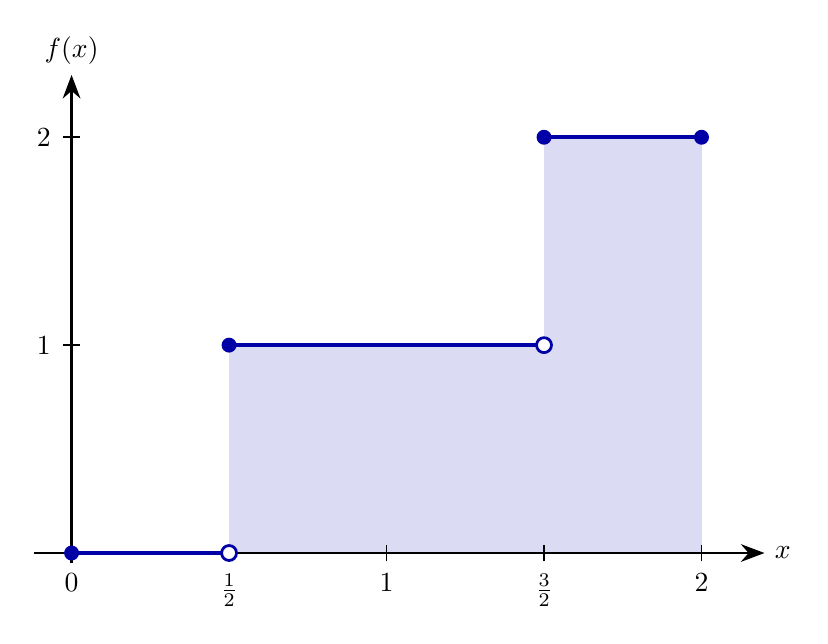
\begin{tikzpicture}[x=4cm,y=2.64cm]
\colorlet{stepblue}{blue!65!black}
\def\half{0.5}
\pgfmathsetmacro{\one}{2*(\half)}
\pgfmathsetmacro{\threehalf}{3*(\half)}
\pgfmathsetmacro{\two}{4*(\half)}
\def\xmin{-0.12}
\def\xmax{2.2}
\def\ymin{-0.05}
\def\ymax{2.3}

\coordinate (O) at (0,0);
\coordinate (A) at (\half,0);
\coordinate (B) at (\half,\one);
\coordinate (M) at (\one,0);
\coordinate (N) at (\one,\one);
\coordinate (C) at (\threehalf,\one);
\coordinate (D) at (\threehalf,0);
\coordinate (E) at (\threehalf,\two);
\coordinate (F) at (\two,\two);

\fill[stepblue!14] (A) rectangle (N);
\fill[stepblue!14] (M) rectangle (C);
\fill[stepblue!14] (D) rectangle (F);

\draw[thick,black,-{Stealth[length=3mm]}]
    (\xmin,0) -- (\xmax,0) node[right] {$x$};
\draw[thick,black,-{Stealth[length=3mm]}]
    (0,\ymin) -- (0,\ymax) node[above] {$f(x)$};

\foreach \n/\lab in {0/0,1/{\frac{1}{2}},2/1,3/{\frac{3}{2}},4/2} {
    \coordinate (xtick) at ({(\n)*(\half)},0);
    \draw[semithick,black] ([yshift=-3pt]xtick) -- ([yshift=3pt]xtick);
    \node[below,yshift=-4pt] at (xtick) {$\lab$};
}
\foreach \n in {1,2} {
    \coordinate (ytick) at (0,\n);
    \draw[semithick,black] ([xshift=-3pt]ytick) -- ([xshift=3pt]ytick);
    \node[left,xshift=-4pt] at (ytick) {$\n$};
}

\draw[stepblue,line width=1.6pt] (O) -- (A);
\draw[stepblue,line width=1.6pt] (B) -- (C);
\draw[stepblue,line width=1.6pt] (E) -- (F);

\foreach \p in {O,B,E,F} {
    \fill[stepblue] (\p) circle[radius=2.7pt];
}
\foreach \p in {A,C} {
    \filldraw[fill=white,draw=stepblue,line width=1pt]
        (\p) circle[radius=2.7pt];
}
\end{tikzpicture}
% end q000156 figure F1
\end{djsSolutionFigure}

Values at isolated endpoints do not affect the integral, because a single point has no width. Adding the three rectangle areas gives
\[
\begin{aligned}
\int_0^2 f(x)\,\mathrm{d}x
&=0\times\frac12+1\times1+2\times\frac12\\[8pt]
&=1+1=\boxed{2}
\end{aligned}
\]

The correct option is \textbf{E}.
% end q000156 solution
\end{djsSolution}
\end{enumerate}
\clearpage
\thispagestyle{djssolutions}
\vspace*{8pt}
\djsTopicLine{Logic}
\begin{enumerate}[label=\textbf{\arabic*.},leftmargin=*,itemsep=0pt,start=10]
\questionitem[Logic]
% begin q000782 stem
Let $f$ be a polynomial defined for all real numbers $x$.

Let $g$ be the function defined by
\[
g(x) = \int_0^x f(t)\,\mathrm{d}t
\]
for all real numbers $x$.

Consider the following three conditions on $f$:
\[
\begin{array}{@{}ll@{}}
\textbf{1} & x f(x) \ge 0\text{ for all real numbers }x \\[5pt]
\textbf{2} & g(x) \ge 0\text{ for all real numbers }x \\[5pt]
\textbf{3} & f(0) = 0\\[5pt]
\end{array}
\]
Consider also the following three statements:
\[
\begin{array}{@{}ll@{}}
\textbf{I} & \text{Condition 1 is necessary for Condition 2} \\[5pt]
\textbf{II} & \text{Condition 1 is sufficient for Condition 2} \\[5pt]
\textbf{III} & \text{Condition 3 is necessary for Condition 2} \\[5pt]
\end{array}
\]
Which of the statements I, II and III is/are true?
% end q000782 stem

\par\vspace*{12pt}
\begin{tabularx}{\linewidth}{@{}>{\bfseries}l Y@{}}
A &
% begin q000782 choice A
None of them
% end q000782 choice A
\\[0.8em]
B &
% begin q000782 choice B
I only
% end q000782 choice B
\\[0.8em]
C &
% begin q000782 choice C
II only
% end q000782 choice C
\\[0.8em]
D &
% begin q000782 choice D
III only
% end q000782 choice D
\\[0.8em]
E &
% begin q000782 choice E
I and II only
% end q000782 choice E
\\[0.8em]
F &
% begin q000782 choice F
I and III only
% end q000782 choice F
\\[0.8em]
G &
% begin q000782 choice G
II and III only
% end q000782 choice G
\\[0.8em]
H &
% begin q000782 choice H
I, II and III
% end q000782 choice H
\\
\end{tabularx}

\begin{djsSolution}{G}
% begin q000782 solution
By the Fundamental Theorem of Calculus,
\[
\frac{\mathrm{d}}{\mathrm{d}x}\int_a^x f(t)\,\mathrm{d}t=f(x)
\]

Applying this to $g$, and evaluating its integral at $0$, gives
\[
g'(x)=f(x)\qquad\text{and}\qquad g(0)=0
\]

For non-zero $x$, Condition 1 requires $f(x)$ to have the same sign as $x$, or to be zero. Thus it means
\[
f(x)\geq0\text{ for }x>0
\qquad\text{and}\qquad
f(x)\leq0\text{ for }x<0
\]

Statement I says: if $g(x)\geq0$ for every real $x$, then $xf(x)\geq0$ for every real $x$. To disprove it, we need a polynomial whose accumulated integral is always non-negative, but whose sign fails the requirement above somewhere.

A cubic can be negative for $x<0$, rise to a large positive local maximum for $x>0$, then dip only slightly below the axis before rising to infinity. The sketch shows such a cubic.

\begin{djsSolutionFigure}
% begin q000782 figure F1
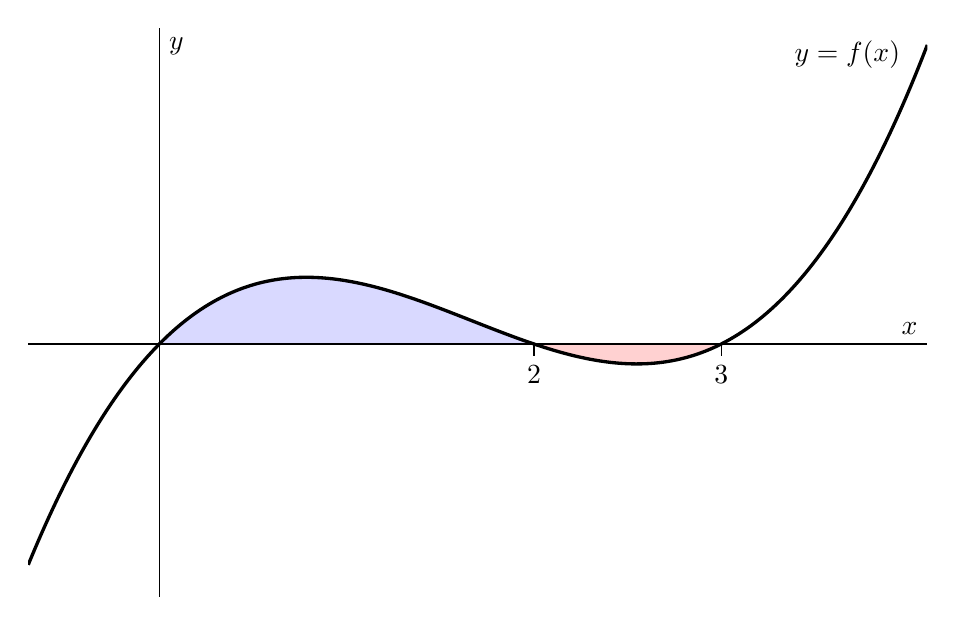
\begin{tikzpicture}
\def\rootB{2}
\def\rootC{3}
\begin{axis}[
    width=13cm, height=8.8cm,
    xmin=-0.7, xmax=4.1,
    ymin=-8, ymax=10,
    axis lines=middle,
    axis line style={thin, black, -},
    axis on top,
    xlabel={$x$}, ylabel={$y$},
    xtick={\rootB,\rootC},
    xticklabels={$2$,$3$},
    ytick=\empty,
    minor tick num=0,
    tick align=outside,
    tick style={thin, black},
    clip=true,
    clip mode=individual
]
\addplot[draw=none, name path=positiveCurve, domain=0:\rootB, samples=100]
    {x*(x-(\rootB))*(x-(\rootC))};
\addplot[draw=none, name path=positiveAxis, domain=0:\rootB, samples=2] {0};
\addplot[draw=none, fill=blue!15]
    fill between[of=positiveCurve and positiveAxis];
\addplot[draw=none, name path=negativeCurve, domain=\rootB:\rootC, samples=80]
    {x*(x-(\rootB))*(x-(\rootC))};
\addplot[draw=none, name path=negativeAxis, domain=\rootB:\rootC, samples=2] {0};
\addplot[draw=none, fill=red!18]
    fill between[of=negativeCurve and negativeAxis];
\addplot[very thick, black, domain=-0.7:4.1, samples=220]
    {x*(x-(\rootB))*(x-(\rootC))}
    node[pos=0.95, above left, inner sep=4pt] {$y=f(x)$};
\end{axis}
\end{tikzpicture}
% end q000782 figure F1
\end{djsSolutionFigure}

The positive shaded area is larger than the negative shaded area, so the negative dip never cancels all the positive area already accumulated. For $x<0$, integrating the negative part of $f$ with reversed limits also gives a non-negative result.

This graphical picture explains why Statement I need not hold; finding a formula is not essential to the argument. For completeness, the cubic drawn is
\[
f(x)=x(x-2)(x-3)=x^3-5x^2+6x
\]

Its integral verifies that Condition 2 holds everywhere:
\[
\begin{aligned}
g(x)&=\frac{x^4}{4}-\frac{5x^3}{3}+3x^2\\[8pt]
&=x^2\left(\frac{x^2}{4}-\frac{5x}{3}+3\right)\\[8pt]
&=x^2\left(\frac14\left(x-\frac{10}{3}\right)^2+\frac29\right)\geq0
\end{aligned}
\]

However, at the positive value $x=\frac52$,
\[
f\left(\frac52\right)=\frac52\times\frac12\times\left(-\frac12\right)=-\frac58<0
\]

Condition 1 therefore fails, so Statement I is false.

Statement II says: if $xf(x)\geq0$ for every real $x$, then $g(x)\geq0$ for every real $x$. For $x>0$, the integral contains only non-negative values of $f$, so
\[
g(x)=\int_0^x f(t)\,\mathrm{d}t\geq0
\]

For $x<0$, $f(t)\leq0$ between $x$ and $0$, so the integral from $x$ to $0$ is non-positive. Reversing the limits changes the sign of an integral, giving
\[
g(x)=\int_0^x f(t)\,\mathrm{d}t
=-\int_x^0 f(t)\,\mathrm{d}t\geq0
\]

Together with $g(0)=0$, this proves Condition 2 for every real $x$. Statement II is true.

Statement III says: if $g(x)\geq0$ for every real $x$, then $f(0)=0$. Since $g(0)=0$, Condition 2 makes $x=0$ a minimum of the differentiable function $g$.

The derivative at this minimum is zero, so
\[
g'(0)=0\implies f(0)=0
\]

Statement III is true. Hence the true statements are
\[
\boxed{\text{II and III only}}
\]

The correct option is \textbf{G}.\\[5pt]

\textit{Alternative Solution:}

For Statement I, we can construct a counterexample by starting with a non-negative polynomial $g$ and then finding $f=g'$. Choose
\[
g(x)=x^2(x-3)^2=x^4-6x^3+9x^2
\]

This is non-negative for every real $x$ and has $g(0)=0$. Differentiating gives
\[
f(x)=g'(x)=4x^3-18x^2+18x
\]

This choice also satisfies the required integral relationship:
\[
\int_0^x f(t)\,\mathrm{d}t
=\left[t^4-6t^3+9t^2\right]_0^x
=x^2(x-3)^2=g(x)
\]

The graph remains on or above the axis, with minima at $0$ and $3$, but it decreases between $\frac32$ and $3$. In particular, its downward tangent at $x=2$ shows how $f(2)=g'(2)$ can be negative while $g$ remains non-negative.

\begin{djsSolutionFigure}
% begin q000782 figure F2
\begin{tikzpicture}
\def\root{3}
\pgfmathsetmacro{\turningX}{(\root)/2}
\def\tangentX{2}
\pgfmathsetmacro{\tangentY}{(\tangentX)^2*((\tangentX)-(\root))^2}
\pgfmathsetmacro{\tangentSlope}{2*(\tangentX)*((\tangentX)-(\root))*(2*(\tangentX)-(\root))}
\pgfmathsetmacro{\leftX}{(\tangentX)-0.65}
\pgfmathsetmacro{\rightX}{(\tangentX)+0.65}
\pgfmathsetmacro{\leftY}{(\tangentY)+(\tangentSlope)*((\leftX)-(\tangentX))}
\pgfmathsetmacro{\rightY}{(\tangentY)+(\tangentSlope)*((\rightX)-(\tangentX))}
\begin{axis}[
    width=13cm, height=8.8cm,
    xmin=-0.65, xmax=3.7,
    ymin=-0.6, ymax=7.5,
    axis lines=middle,
    axis line style={thin, black, -},
    xlabel={$x$}, ylabel={$y$},
    xtick={\turningX,\tangentX,\root},
    xticklabels={$\frac{3}{2}$,$2$,$3$},
    ytick=\empty,
    minor tick num=0,
    tick align=outside,
    tick style={thin, black},
    clip=true,
    clip mode=individual
]
\addplot[thick, blue!65!black, domain=-0.65:3.7, samples=240]
    {x^2*(x-(\root))^2}
    node[pos=0.975, above left, text=blue!65!black, inner sep=4pt] {$y=g(x)$};
\addplot[line width=1.7pt, red!70!black, domain=\turningX:\root, samples=100]
    {x^2*(x-(\root))^2};
\coordinate (TLeft) at (axis cs:\leftX,\leftY);
\coordinate (TRight) at (axis cs:\rightX,\rightY);
\coordinate (TPoint) at (axis cs:\tangentX,\tangentY);
\draw[black, thick, dashed,
    postaction={decorate},
    decoration={markings, mark=at position 0.28 with {\arrow{Stealth[length=2mm]}}}
] (TLeft) -- (TRight);
\fill[black] (TPoint) circle[radius=1.6pt];
\node[below left, inner sep=3pt] at (axis cs:0,0) {$0$};
\end{axis}
\end{tikzpicture}
% end q000782 figure F2
\end{djsSolutionFigure}

Explicitly,
\[
f(2)=4(2)^3-18(2)^2+18(2)=32-72+36=-4
\]

Thus $2f(2)=-8<0$: Condition 2 holds, but Condition 1 fails. Statement I is false, and the arguments above establish that II and III are true, again giving option \textbf{G}.
% end q000782 solution
\end{djsSolution}
\end{enumerate}
\clearpage
\thispagestyle{djssolutions}
\vspace*{8pt}
\djsTopicLine{Number}
\begin{enumerate}[label=\textbf{\arabic*.},leftmargin=*,itemsep=0pt,start=11]
\questionitem[Number]
% begin q000734 stem
Let $N=2^8\times3^6$ 

A positive integer $k$ is called \textit{suitable} if both $\dfrac{N}{k^2}$ and $\dfrac{k^3}{N}$ are integers. 

What is the sum of all suitable values of $k$?
% end q000734 stem

\par\vspace*{12pt}
\begin{tabularx}{\linewidth}{@{}>{\bfseries}l Y@{}}
A &
% begin q000734 choice A
$432$
% end q000734 choice A
\\[0.8em]
B &
% begin q000734 choice B
$576$
% end q000734 choice B
\\[0.8em]
C &
% begin q000734 choice C
$648$
% end q000734 choice C
\\[0.8em]
D &
% begin q000734 choice D
$864$
% end q000734 choice D
\\[0.8em]
E &
% begin q000734 choice E
$1296$
% end q000734 choice E
\\
\end{tabularx}

\begin{djsSolution}{D}
% begin q000734 solution
Since $N/k^2$ is an integer, $k^2$ is a factor of $N$. Hence $k$ has no prime factors other than $2$ and $3$, so write $k=2^a3^b$, where $a$ and $b$ are non-negative integers.

The two quotients are
\[
\begin{aligned}
\frac{N}{k^2}&=2^{8-2a}3^{6-2b}\\[8pt]
\frac{k^3}{N}&=2^{3a-8}3^{3b-6}
\end{aligned}
\]

Each quotient is an integer exactly when both of its prime exponents are non-negative. For the first quotient, this requires
\[
8-2a\geq0\quad\text{and}\quad6-2b\geq0
\implies a\leq4\quad\text{and}\quad b\leq3
\]

For the second quotient, it requires
\[
3a-8\geq0\quad\text{and}\quad3b-6\geq0
\implies a\geq\frac83\quad\text{and}\quad b\geq2
\]

Intersecting these conditions and using the fact that the exponents are integers gives
\[
\begin{aligned}
\frac83\leq a\leq4&\implies a=3\text{ or }a=4\\[8pt]
2\leq b\leq3&\implies b=2\text{ or }b=3
\end{aligned}
\]

Every combination of these exponents makes both quotients integers. Thus the complete list of suitable values is
\[
\begin{array}{c|c|c}
a&b&k=2^a3^b\\[5pt]
\hline
\rule{0pt}{2.5ex}3&2&2^3\times3^2=72\\[5pt]
3&3&2^3\times3^3=216\\[5pt]
4&2&2^4\times3^2=144\\[5pt]
4&3&2^4\times3^3=432
\end{array}
\]

Their sum is
\[
72+216+144+432=288+576=\boxed{864}
\]

The correct option is \textbf{D}.
% end q000734 solution
\end{djsSolution}
\end{enumerate}
\clearpage
\thispagestyle{djssolutions}
\vspace*{8pt}
\djsTopicLine{Proof \& Error Analysis}
\begin{enumerate}[label=\textbf{\arabic*.},leftmargin=*,itemsep=0pt,start=12]
\questionitem[Proof \& Error Analysis]
% begin q000786 stem
In this question you may use the facts \[\sin\dfrac{\pi}{12}=\dfrac{\sqrt{6}-\sqrt{2}}{4} \qquad\text{and}\qquad\sin\dfrac{5\pi}{12}=\dfrac{\sqrt{6}+\sqrt{2}}{4}\] \vspace*{5pt}


A student attempts to answer the following question.

\begin{center}
\begin{minipage}{0.82\linewidth}
\centering
Find all real values of $x$, with $0<x<\pi$, such that $\log_{2}(\sin x)+\log_{2}(\cos x)=-2$.
\end{minipage}
\end{center}

The student's attempt is as follows.

\[
\begin{array}{@{}ll@{}}
\textbf{I} & \text{Using the laws of logarithms, the equation becomes } \log_{2}(\sin x\cos x)=-2 \\[10pt]
\textbf{II} & \text{Hence } \sin x\cos x=\dfrac{1}{4} \\[10pt]
\textbf{III} & \text{Every solution must therefore satisfy } \sin^{2}x\cos^{2}x=\dfrac{1}{16} \\[10pt]
\textbf{IV} & \text{Writing}\ \cos^{2}x=1-\sin^{2}x\ \text{and}\ s=\sin^{2}x\text{ this becomes } 16s^{2}-16s+1=0 \\[10pt]
\textbf{V} & \text{Hence every solution must have } s=\dfrac{2\pm\sqrt{3}}{4}\text{, and since}\\[8pt]& \sin x>0\ \text{for}\ 0<x<\pi\text{,}\, \sin x=\dfrac{\sqrt{6}\pm\sqrt{2}}{4} \\[10pt]
\textbf{VI} & \text{Therefore } x=\dfrac{\pi}{12},\ \dfrac{5\pi}{12},\ \dfrac{7\pi}{12},\dfrac{11\pi}{12} \\[10pt]
\end{array}
\]

Which of the following best describes the attempt?
% end q000786 stem

\par\vspace*{12pt}
\begin{tabularx}{\linewidth}{@{}>{\bfseries}l Y@{}}
A &
% begin q000786 choice A
The attempt is completely correct.
% end q000786 choice A
\\[0.8em]
B &
% begin q000786 choice B
The attempt is incorrect, and the first error occurs in line I.
% end q000786 choice B
\\[0.8em]
C &
% begin q000786 choice C
The attempt is incorrect, and the first error occurs in line III.
% end q000786 choice C
\\[0.8em]
D &
% begin q000786 choice D
The attempt is incorrect, and the first error occurs in line IV.
% end q000786 choice D
\\[0.8em]
E &
% begin q000786 choice E
The attempt is incorrect, and the first error occurs in line V.
% end q000786 choice E
\\[0.8em]
F &
% begin q000786 choice F
The attempt is incorrect, and the first error occurs in line VI.
% end q000786 choice F
\\
\end{tabularx}

\begin{djsSolution}{F}
% begin q000786 solution
The attempt ends with proposed solutions, so test one in the original equation before locating the first error. Choose $x=\frac{7\pi}{12}$, which lies in the second quadrant:
\[
\cos\frac{7\pi}{12}=-\sin\frac{\pi}{12}=-\frac{\sqrt6-\sqrt2}{4}<0
\]

Thus $\log_2(\cos x)$ is not defined as a real number for this value. The proposed list therefore contains a false solution.

Now check the lines in order to locate the first error.

The original equation requires $\sin x>0$ and $\cos x>0$. On this domain, the law $\log_2 a+\log_2 b=\log_2(ab)$ gives line I, so line I is correct.

For line II, the definition of a logarithm gives
\[
\log_2(\sin x\cos x)=-2
\implies \sin x\cos x=2^{-2}=\frac14
\]

Line II is correct.

In line III, ``every solution must'' means that if $x$ solves the original equation, then it satisfies the squared equation. Squaring line II gives
\[
\sin^2x\cos^2x=\left(\frac14\right)^2=\frac1{16}
\]

Line III is correct: it gives a necessary condition, not a guarantee that every solution of the squared equation solves the original equation. Squaring loses the distinction between a product of $\frac14$ and a product of $-\frac14$.

For line IV, using $\sin^2x+\cos^2x=1$ and writing $s=\sin^2x$ gives
\[
s(1-s)=\frac1{16}
\implies 16s-16s^2=1
\implies 16s^2-16s+1=0
\]

Line IV is correct.

For line V, the quadratic formula gives
\[
s=\frac{16\pm\sqrt{(-16)^2-4(16)(1)}}{2(16)}
=\frac{16\pm8\sqrt3}{32}
=\frac{2\pm\sqrt3}{4}
\]

The quickest way to check the stated square roots is to square them:
\[
\left(\frac{\sqrt6\pm\sqrt2}{4}\right)^2
=\frac{8\pm4\sqrt3}{16}
=\frac{2\pm\sqrt3}{4}
\]

Both proposed square roots are positive, and $\sin x>0$ for $0<x<\pi$. Hence line V correctly concludes that every solution must have
\[
\sin x=\frac{\sqrt6-\sqrt2}{4}
\quad\text{or}\quad
\sin x=\frac{\sqrt6+\sqrt2}{4}
\]

The first error is in line VI. It accepts every candidate from the necessary conditions without checking the original equation.

For example, the value tested above does satisfy line V:
\[
\sin\frac{7\pi}{12}
=\sin\frac{5\pi}{12}
=\frac{\sqrt6+\sqrt2}{4}
\]

However, its cosine is negative, so it cannot solve the original logarithmic equation. The correct option is \textbf{F}.\\[5pt]

\textit{Remark:}

To repair line VI, enforce the positive logarithm arguments. Within $0<x<\pi$, the sine is positive, but the cosine is positive only for $0<x<\frac\pi2$, leaving the candidates $x=\frac\pi{12}$ and $x=\frac{5\pi}{12}$.

Complementary angles give
\[
\cos\frac\pi{12}=\sin\frac{5\pi}{12}
\qquad\text{and}\qquad
\cos\frac{5\pi}{12}=\sin\frac\pi{12}
\]

Using the supplied sine values, both candidates satisfy line II:
\[
\begin{aligned}
\sin\frac\pi{12}\cos\frac\pi{12}
&=\sin\frac{5\pi}{12}\cos\frac{5\pi}{12}\\[8pt]
&=\frac{\sqrt6-\sqrt2}{4}\times\frac{\sqrt6+\sqrt2}{4}
=\frac{6-2}{16}=\frac14
\end{aligned}
\]

Both logarithm arguments are positive, so for each candidate
\[
\log_2(\sin x)+\log_2(\cos x)
=\log_2(\sin x\cos x)
=\log_2\frac14=-2
\]

The repaired list of solutions is therefore
\[
x=\frac\pi{12}\quad\text{or}\quad x=\frac{5\pi}{12}
\]
% end q000786 solution
\end{djsSolution}
\end{enumerate}
\clearpage
\thispagestyle{djssolutions}
\vspace*{8pt}
\djsTopicLine{Number}
\begin{enumerate}[label=\textbf{\arabic*.},leftmargin=*,itemsep=0pt,start=13]
\questionitem[Number]
% begin q000730 stem
There is a non-negative integer $k$ such that the binomial coefficient $\dbinom{64}{32}$ is divisible by $2^k$ but not by $2^{k+1}$ 

What is the value of $k$?
% end q000730 stem

\par\vspace*{12pt}
\begin{tabularx}{\linewidth}{@{}>{\bfseries}l Y@{}}
A &
% begin q000730 choice A
$0$
% end q000730 choice A
\\[0.8em]
B &
% begin q000730 choice B
$1$
% end q000730 choice B
\\[0.8em]
C &
% begin q000730 choice C
$2$
% end q000730 choice C
\\[0.8em]
D &
% begin q000730 choice D
$16$
% end q000730 choice D
\\[0.8em]
E &
% begin q000730 choice E
$31$
% end q000730 choice E
\\[0.8em]
F &
% begin q000730 choice F
$32$
% end q000730 choice F
\\[0.8em]
G &
% begin q000730 choice G
$63$
% end q000730 choice G
\\
\end{tabularx}

\begin{djsSolution}{B}
% begin q000730 solution
Using the binomial coefficient formula
\[
\binom{n}{r}=\frac{n!}{r!(n-r)!}
\]
we have
\[
\binom{64}{32}=\frac{64!}{(32!)^2}
\]

We need to count the factors of $2$ in the numerator and denominator, rather than calculate the coefficient itself.

In a factorial, each multiple of $2$ contributes one factor of $2$, each multiple of $4$ contributes an additional factor, each multiple of $8$ contributes another, and so on. This repeated counting gives each term its full number of factors of $2$: for example, $8$ is counted among the multiples of $2$, $4$ and $8$.

The exponents of $2$ in the two factorials are therefore
\[
\begin{aligned}
\text{Exponent in }64!&=32+16+8+4+2+1=63\\[5pt]
\text{Exponent in }32!&=16+8+4+2+1=31
\end{aligned}
\]

There are two copies of $32!$ in the denominator, so the exponent remaining after division is
\[
k=63-2(31)=\boxed{1}
\]

The coefficient is divisible by $2$ but not by $4$, so the correct option is \textbf{B}.\\[5pt]

\textit{Alternative Solution:}

Cancelling one copy of $32!$ first gives
\[
\binom{64}{32}
=\frac{33\cdot34\cdots64}{1\cdot2\cdots32}
=\frac{64}{32}\times\frac{33\cdot34\cdots63}{1\cdot2\cdots31}
=2\times\frac{33\cdot34\cdots63}{1\cdot2\cdots31}
\]

Pair each denominator term $i$ with the numerator term $32+i$, for $1\leq i\leq31$. We will show that the two terms in each pair contain equally many factors of $2$.

Write $i=2^a m$, where $m$ is odd and $a$ is a non-negative integer. Since $i<32=2^5$, we have $a<5$, and
\[
32+i=2^5+2^a m=2^a\bigl(2^{5-a}+m\bigr)
\]

Because $a<5$, the number $2^{5-a}$ is even, so $2^{5-a}+m$ is odd. Thus both $i$ and $32+i$ contain exactly $a$ factors of $2$.

Removing these matching powers of $2$ from every pair leaves an odd numerator and an odd denominator. The only remaining factor of $2$ is the initial factor from $64/32$.

Cancelling an odd denominator cannot remove that factor of $2$ or introduce another one. Since the binomial coefficient is an integer, it is twice an odd integer, again giving option \textbf{B}.
% end q000730 solution
\end{djsSolution}
\end{enumerate}
\clearpage
\thispagestyle{djssolutions}
\vspace*{8pt}
\djsTopicLine{Probability \& Counting}
\begin{enumerate}[label=\textbf{\arabic*.},leftmargin=*,itemsep=0pt,start=14]
\questionitem[Probability \& Counting]
% begin q000781 stem
Two cards are drawn in order, without replacement, from cards numbered $1$ to $6$. 

Consider the events
\[
\begin{array}{@{}ll@{}}
\textbf{A} & \text{The first card has an even number} \\[5pt]
\textbf{B} & \text{The second card has an even number} \\[5pt]
\textbf{C} & \text{The sum of the two numbers is odd} \\[5pt]
\end{array}
\]

We say that two events are \emph{independent} if the probability that both occur is equal to their individual probabilities multiplied together.

In notation, \[A \text{ and } B \text{ are independent} \quad\iff\quad P(A \text{ and } B) = P(A)\times P(B)\]

Which pairs of the events $A, B$ and $C$ are independent?
% end q000781 stem

\par\vspace*{12pt}
\begin{tabularx}{\linewidth}{@{}>{\bfseries}l Y@{}}
A &
% begin q000781 choice A
None of the three pairs
% end q000781 choice A
\\[0.8em]
B &
% begin q000781 choice B
$A$ and $B$ only
% end q000781 choice B
\\[0.8em]
C &
% begin q000781 choice C
$A$ and $C$ only
% end q000781 choice C
\\[0.8em]
D &
% begin q000781 choice D
$B$ and $C$ only
% end q000781 choice D
\\[0.8em]
E &
% begin q000781 choice E
$A$ and $C$; $B$ and $C$
% end q000781 choice E
\\
\end{tabularx}

\begin{djsSolution}{E}
% begin q000781 solution
For each pair, compare the probability that both events occur with the product of their individual probabilities. The pair is independent exactly when these are equal.

There are three even cards and three odd cards, so the first card is even or odd with probability $\frac12$ each. After the first draw, there are two cards of the same parity as the first card and three of the opposite parity.

Multiplying the branch probabilities along each route gives the four probabilities shown at the ends of the tree.

\begin{djsSolutionFigure}
% begin q000781 figure F1
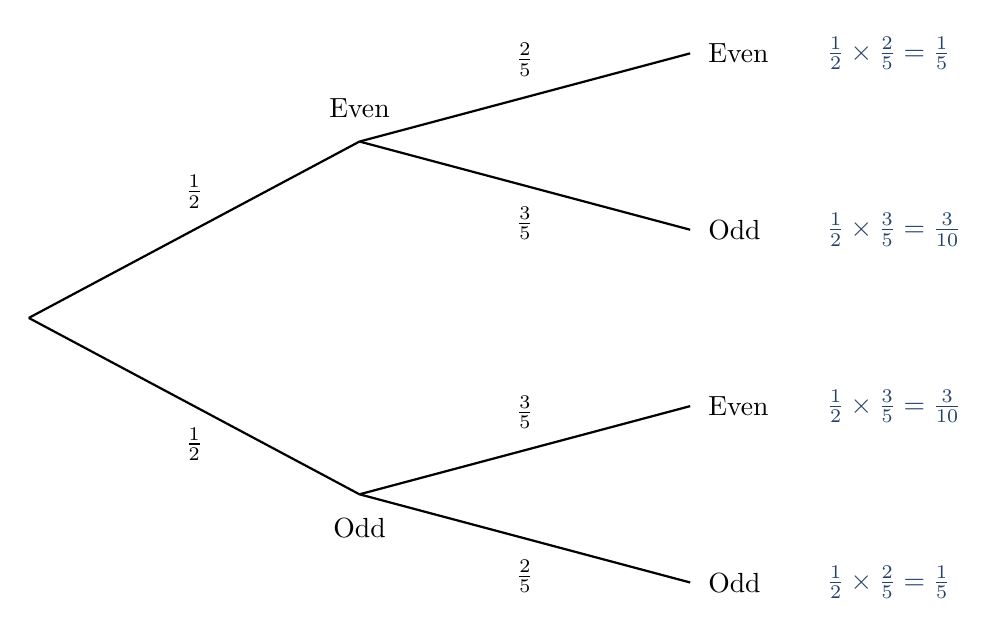
\begin{tikzpicture}[x=1.4cm,y=1.4cm]
\definecolor{routeblue}{RGB}{35,65,105}
\def\firstx{3}
\def\firstheight{1.6}
\def\terminalx{6}
\def\splitheight{0.8}
\def\calculationoffset{1.15}
\coordinate (Root) at (0,0);
\coordinate (FirstEven) at (\firstx,\firstheight);
\coordinate (FirstOdd) at (\firstx,-\firstheight);
\coordinate (EE) at (\terminalx,{(\firstheight)+(\splitheight)});
\coordinate (EO) at (\terminalx,{(\firstheight)-(\splitheight)});
\coordinate (OE) at (\terminalx,{-(\firstheight)+(\splitheight)});
\coordinate (OO) at (\terminalx,{-(\firstheight)-(\splitheight)});

\draw[thick,black] (Root) -- node[midway,above=4pt] {$\frac12$} (FirstEven);
\draw[thick,black] (Root) -- node[midway,below=4pt] {$\frac12$} (FirstOdd);
\draw[thick,black] (FirstEven) -- node[midway,above=4pt] {$\frac25$} (EE);
\draw[thick,black] (FirstEven) -- node[midway,below=4pt] {$\frac35$} (EO);
\draw[thick,black] (FirstOdd) -- node[midway,above=4pt] {$\frac35$} (OE);
\draw[thick,black] (FirstOdd) -- node[midway,below=4pt] {$\frac25$} (OO);

\node[above=5pt] at (FirstEven) {Even};
\node[below=5pt] at (FirstOdd) {Odd};
\node[right=3pt] at (EE) {Even};
\node[right=3pt] at (EO) {Odd};
\node[right=3pt] at (OE) {Even};
\node[right=3pt] at (OO) {Odd};

\node[anchor=west,text=routeblue] at ($(EE)+(\calculationoffset,0)$) {$\frac12\times\frac25=\frac15$};
\node[anchor=west,text=routeblue] at ($(EO)+(\calculationoffset,0)$) {$\frac12\times\frac35=\frac3{10}$};
\node[anchor=west,text=routeblue] at ($(OE)+(\calculationoffset,0)$) {$\frac12\times\frac35=\frac3{10}$};
\node[anchor=west,text=routeblue] at ($(OO)+(\calculationoffset,0)$) {$\frac12\times\frac25=\frac15$};
\end{tikzpicture}
% end q000781 figure F1
\end{djsSolutionFigure}

Event $C$ occurs exactly when one card is even and the other is odd. Adding the relevant route probabilities gives
\[
\begin{aligned}
P(A)&=\frac15+\frac3{10}=\frac12\\[8pt]
P(B)&=\frac15+\frac3{10}=\frac12\\[8pt]
P(C)&=\frac3{10}+\frac3{10}=\frac35
\end{aligned}
\]

Now test each pair. Events $A$ and $B$ occur together only on the even-then-even route, so
\[
P(A\text{ and }B)=\frac15
\qquad\text{but}\qquad
P(A)\times P(B)=\frac12\times\frac12=\frac14
\]

The probabilities are unequal, so $A$ and $B$ are not independent.

Events $A$ and $C$ occur together only on the even-then-odd route. Here
\[
P(A)\times P(C)=\frac12\times\frac35=\frac3{10}=P(A\text{ and }C)
\]

Thus $A$ and $C$ are independent.

Events $B$ and $C$ occur together only on the odd-then-even route. Here
\[
P(B)\times P(C)=\frac12\times\frac35=\frac3{10}=P(B\text{ and }C)
\]

Thus $B$ and $C$ are also independent, so the correct option is \textbf{E}.
% end q000781 solution
\end{djsSolution}
\end{enumerate}
\clearpage
\thispagestyle{djssolutions}
\vspace*{8pt}
\djsTopicLine{Probability \& Counting}
\begin{enumerate}[label=\textbf{\arabic*.},leftmargin=*,itemsep=0pt,start=15]
\questionitem[Probability \& Counting]
% begin q000780 stem
A positive integer is called \emph{ascending} if it has at least two digits and, reading its digits from left to right, each digit is strictly greater than the one before it. 

For example, $259$ is ascending, but $2556$ and $92$ are not.

How many ascending integers are there less than $10000$?
% end q000780 stem

\par\vspace*{12pt}
\begin{tabularx}{\linewidth}{@{}>{\bfseries}l Y@{}}
A &
% begin q000780 choice A
$126$
% end q000780 choice A
\\[0.8em]
B &
% begin q000780 choice B
$210$
% end q000780 choice B
\\[0.8em]
C &
% begin q000780 choice C
$246$
% end q000780 choice C
\\[0.8em]
D &
% begin q000780 choice D
$255$
% end q000780 choice D
\\[0.8em]
E &
% begin q000780 choice E
$375$
% end q000780 choice E
\\[0.8em]
F &
% begin q000780 choice F
$495$
% end q000780 choice F
\\[0.8em]
G &
% begin q000780 choice G
$3600$
% end q000780 choice G
\\
\end{tabularx}

\begin{djsSolution}{C}
% begin q000780 solution
An ascending integer cannot contain $0$: it would have to be the first digit, since all subsequent digits must be larger. An integer cannot begin with $0$.

The available digits are therefore $1$ to $9$, and an ascending integer less than $10000$ has exactly $2$, $3$ or $4$ digits.

Each choice of distinct digits gives exactly one ascending integer, by putting those digits in increasing order. Conversely, every ascending integer is obtained this way, so choosing the digits counts every ascending integer exactly once.

The number of ways to choose $r$ digits from $n$ distinct digits is
\[
\binom{n}{r}=\frac{n!}{r!(n-r)!}
\]

Counting separately by digit length gives
\[
\begin{aligned}
\text{Two digits:}\quad \binom{9}{2}&=\frac{9\times8}{2\times1}=36\\[8pt]
\text{Three digits:}\quad \binom{9}{3}&=\frac{9\times8\times7}{3\times2\times1}=84\\[8pt]
\text{Four digits:}\quad \binom{9}{4}&=\frac{9\times8\times7\times6}{4\times3\times2\times1}=126
\end{aligned}
\]

These three cases do not overlap, so the total is
\[
36+84+126=\boxed{246}
\]

The correct option is \textbf{C}.
% end q000780 solution
\end{djsSolution}
\end{enumerate}
\clearpage
\thispagestyle{djssolutions}
\vspace*{8pt}
\djsTopicLine{Number}
\begin{enumerate}[label=\textbf{\arabic*.},leftmargin=*,itemsep=0pt,start=16]
\questionitem[Number]
% begin q000007 stem
Let $n$ be a positive integer. Consider the following conditions: \[ \begin{array}{@{}l l@{}}
\textbf{I:} & \text{$n$ is even} \\[2pt]
\textbf{II:} & \text{$n$ is a multiple of $3$} \\[2pt]
\textbf{III:} & \text{$n$ is a prime greater than $3$}
\end{array} \] Which of these conditions is/are \textbf{sufficient} for the statement: \[2^n-1 \text{ is divisible by }7\]
% end q000007 stem

\par\vspace*{12pt}
\begin{tabularx}{\linewidth}{@{}>{\bfseries}l Y@{}}
A &
% begin q000007 choice A
I only
% end q000007 choice A
\\[0.8em]
B &
% begin q000007 choice B
II only
% end q000007 choice B
\\[0.8em]
C &
% begin q000007 choice C
III only
% end q000007 choice C
\\[0.8em]
D &
% begin q000007 choice D
I and II only
% end q000007 choice D
\\[0.8em]
E &
% begin q000007 choice E
I and III only
% end q000007 choice E
\\[0.8em]
F &
% begin q000007 choice F
II and III only
% end q000007 choice F
\\[0.8em]
G &
% begin q000007 choice G
I, II, and III
% end q000007 choice G
\\[0.8em]
H &
% begin q000007 choice H
None of them
% end q000007 choice H
\\
\end{tabularx}

\begin{djsSolution}{B}
% begin q000007 solution
A condition is sufficient if, whenever that condition holds, the required statement is true. One example where the condition holds but the statement fails is enough to disprove sufficiency.

For I, we are testing: if $n$ is even, then $2^n-1$ is divisible by $7$. Taking $n=2$ gives
\[
2^2-1=3
\]

This is not divisible by $7$, so I is not sufficient.

For III, we are testing: if $n$ is a prime greater than $3$, then $2^n-1$ is divisible by $7$. Taking $n=5$ gives
\[
2^5-1=32-1=31=7\times4+3
\]

Thus III is not sufficient either.

For II, we must show: if $n$ is a multiple of $3$, then $2^n-1$ is divisible by $7$. This requires $2^n$ to have remainder $1$ when divided by $7$, so tabulate the remainders of successive powers:
\[
\begin{array}{c|rrrrrr}
n&1&2&3&4&5&6\\[5pt]
2^n&2&4&8&16&32&64\\[5pt]
\text{Remainder on division by }7&2&4&1&2&4&1
\end{array}
\]

To justify that this pattern continues, each power is obtained by doubling the previous power. Multiples of $7$ remain multiples of $7$ when doubled, so the next remainder is determined by doubling the previous remainder.

A remainder of $2$ gives $4$; a remainder of $4$ gives $1$, because $2\times4=8=7+1$; and a remainder of $1$ gives $2$. Hence the three-term cycle $2,4,1$ repeats indefinitely.

Whenever $n=3,6,9,\ldots$, the remainder of $2^n$ is therefore $1$, so subtracting $1$ gives a multiple of $7$. Thus the sufficient conditions are
\[
\boxed{\text{II only}}
\]

The correct option is \textbf{B}.\\[5pt]

\textit{Alternative Solution 1:}

The counterexamples $n=2$ and $n=5$ above rule out I and III. To prove II, write $n=3k$, where $k$ is a positive integer.

The finite geometric-series formula is
\[
1+r+\cdots+r^{k-1}=\frac{1-r^k}{1-r}\qquad(r\ne1)
\]

Taking $r=8$ gives
\[
1+8+\cdots+8^{k-1}=\frac{1-8^k}{1-8}=\frac{8^k-1}{7}
\]

Therefore
\[
2^n-1=2^{3k}-1=8^k-1=7\bigl(1+8+\cdots+8^{k-1}\bigr)
\]

The bracket contains $k$ integer terms, so this is divisible by $7$; when $k=1$, the bracket is $1$. Hence II is sufficient, giving option \textbf{B}.\\[5pt]

\textit{Alternative Solution 2:}

This method uses modular arithmetic, which is outside the specification. The notation $a\equiv b\pmod{7}$ means that $a-b$ is divisible by $7$, or equivalently that $a$ and $b$ have the same remainder when divided by $7$.

Congruences can be multiplied: when products are expanded, every term containing a multiple of $7$ is still divisible by $7$. Repeated multiplication therefore allows us to raise both sides of a congruence to a positive integer power.

For II, write $n=3k$, where $k$ is a positive integer. Since
\[
2^3=8\equiv1\pmod{7}
\]
we obtain
\[
2^n-1=(2^3)^k-1\equiv1^k-1=0\pmod{7}
\]

Thus $2^n-1$ is divisible by $7$, proving II sufficient. Together with the counterexamples to I and III above, this again gives option \textbf{B}.
% end q000007 solution
\end{djsSolution}
\end{enumerate}
\clearpage
\thispagestyle{djssolutions}
\vspace*{8pt}
\djsTopicLine{Proof \& Error Analysis}
\begin{enumerate}[label=\textbf{\arabic*.},leftmargin=*,itemsep=0pt,start=17]
\questionitem[Proof \& Error Analysis]
% begin q000151 stem
A statement is given: \[\text{S: For all real numbers $x$, \textbf{if} $x^2 \ge 1$ \textbf{then} $x^4 \ge x^2$}\] A student wishes to prove $S$ by contradiction and writes the following argument:

Assume that there exists a real number $x$ such that $x^2 \ge 1$ \textbf{and} $x^4 < x^2$ \[ \begin{array}{@{}l l@{}}
\textbf{I:} & \text{Then $x^4 - x^2 < 0$} \\[5pt]
\textbf{II:} & \text{So $x^2(x^2 - 1) < 0$} \\[5pt]
\textbf{III:} & \text{So $x^2 - 1 < 0$} \\[5pt]
\textbf{IV:} & \text{So $x^2 < 1$, which contradicts $x^2 \ge 1$}
\end{array} \] Therefore the original statement $S$ is concluded to be true.

Which of the following best describes this argument?
% end q000151 stem

\par\vspace*{12pt}
\begin{tabularx}{\linewidth}{@{}>{\bfseries}l Y@{}}
A &
% begin q000151 choice A
It is completely correct.
% end q000151 choice A
\\[0.8em]
B &
% begin q000151 choice B
It is incorrect, but it would be correct if written in the reverse order.
% end q000151 choice B
\\[0.8em]
C &
% begin q000151 choice C
It is incorrect, and the student has actually shown that $S$ is false.
% end q000151 choice C
\\[0.8em]
D &
% begin q000151 choice D
It is incorrect because line \textbf{II} does not follow from line \textbf{I}.
% end q000151 choice D
\\[0.8em]
E &
% begin q000151 choice E
It is incorrect because line \textbf{III} does not follow from line \textbf{II}.
% end q000151 choice E
\\[0.8em]
F &
% begin q000151 choice F
It is incorrect because the student has not really used proof by contradiction.
% end q000151 choice F
\\
\end{tabularx}

\begin{djsSolution}{A}
% begin q000151 solution
``For all real numbers $x$'' means that the statement must hold for every real value of $x$: if $x^2\ge1$, then $x^4\ge x^2$.

Its negation requires at least one real value of $x$ for which the hypothesis is true and the conclusion is false. The student's assumption is therefore exactly the negation of $S$:
\[
x^2\ge1\qquad\text{and}\qquad x^4<x^2
\]

Multiplying $x^2\ge1$ by the positive number $x^2$ shows that $S$ is true, so there are no counterexamples. However, a true claim can still have an invalid proposed proof, so we must check the student's lines in order.

In line \textbf{I}, subtracting $x^2$ from both sides gives
\[
x^4<x^2\implies x^4-x^2<0
\]

Line \textbf{I} is correct.

In line \textbf{II}, taking out the common factor $x^2$ gives
\[
x^4-x^2=x^2(x^2-1)
\]

The expression is unchanged, so line \textbf{II} is correct.

For line \textbf{III}, the retained assumption $x^2\ge1$ guarantees that $x^2>0$. We can therefore divide by $x^2$ without reversing the inequality:
\[
\frac{x^2(x^2-1)}{x^2}<\frac{0}{x^2}
\implies x^2-1<0
\]

Line \textbf{III} is correct; division by zero is not a risk under the assumption.

In line \textbf{IV}, adding $1$ gives
\[
x^2-1<0\implies x^2<1
\]

This contradicts the assumption $x^2\ge1$, so line \textbf{IV} is correct.

This is proof by contradiction: the student assumes the negation of $S$ and deduces two conditions that cannot both hold. The negation is therefore impossible, and $S$ is true.

The argument is completely correct, so the answer is \textbf{A}.\\[5pt]

\textit{Remark:}

A shorter direct proof starts with $x^2\ge1$ and multiplies both sides by $x^2$, which is positive:
\[
x^2\cdot x^2\ge1\cdot x^2
\implies x^4\ge x^2
\]

This proves the claim itself, whereas checking the student's argument requires establishing that each step and the contradiction are valid.
% end q000151 solution
\end{djsSolution}
\end{enumerate}
\clearpage
\thispagestyle{djssolutions}
\vspace*{8pt}
\djsTopicLine{Integration}
\begin{enumerate}[label=\textbf{\arabic*.},leftmargin=*,itemsep=0pt,start=18]
\questionitem[Integration]
% begin q000622 stem
The region $R$ in the first quadrant is bounded by the curve $y = 4x - x^2$ and the $x$-axis.

The line $y = 2x$ divides $R$ into two sub-regions: $R_1$, which lies above the line, and $R_2$, which lies below the line.

What is the ratio of the area of $R_1$ to the area of $R_2$?
% end q000622 stem

\begin{center}
% begin q000622 diagram
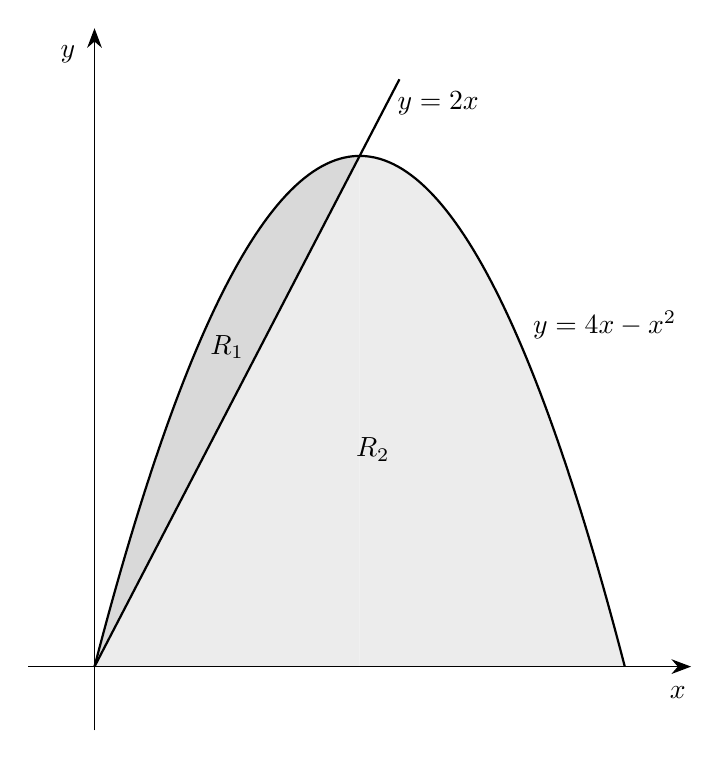
\begin{tikzpicture}
\pgfplotsset{compat=1.18}
\begin{axis}[
    width=10cm,
    height=10.5cm,
    xmin=-0.5, xmax=4.5,
    ymin=-0.5, ymax=5,
    axis lines=middle,
    axis line style={-{Stealth[length=2.5mm]}},
    axis on top,
    xtick=\empty,
    ytick=\empty,
    clip=true,
    samples=120
]
% Exact paths used to shade R_1.
\addplot[draw=none, name path=rOneCurve, domain=0:2]
    {4*x-x^2};
\addplot[draw=none, name path=rOneLine, domain=0:2, samples=2]
    {2*x};
\addplot[gray!30, draw=none]
    fill between[of=rOneCurve and rOneLine];

% Exact component paths used to shade R_2.
\addplot[draw=none, name path=rTwoLine, domain=0:2, samples=2]
    {2*x};
\addplot[draw=none, name path=rTwoAxisA, domain=0:2, samples=2]
    {0};
\addplot[gray!15, draw=none]
    fill between[of=rTwoLine and rTwoAxisA];

\addplot[draw=none, name path=rTwoCurve, domain=2:4]
    {4*x-x^2};
\addplot[draw=none, name path=rTwoAxisB, domain=2:4, samples=2]
    {0};
\addplot[gray!15, draw=none]
    fill between[of=rTwoCurve and rTwoAxisB];

% Boundary curve and dividing line.
\addplot[thick, black, domain=0:4]
    {4*x-x^2}
    node[pos=0.72, above right] {$y=4x-x^2$};
\addplot[thick, black, domain=0:2.3, samples=2]
    {2*x}
    node[pos=0.96, right] {$y=2x$};

% Region and axis labels.
\node at (axis cs:1,2.5) {$R_1$};
\node at (axis cs:2.1,1.7) {$R_2$};
\node at (axis cs:4.4,-0.2) {$x$};
\node at (axis cs:-0.2,4.8) {$y$};
\end{axis}
\end{tikzpicture}
% end q000622 diagram
\end{center}

\par\vspace*{12pt}
\begin{tabularx}{\linewidth}{@{}>{\bfseries}l Y@{}}
A &
% begin q000622 choice A
$1 : 3$
% end q000622 choice A
\\[0.8em]
B &
% begin q000622 choice B
$1 : 4$
% end q000622 choice B
\\[0.8em]
C &
% begin q000622 choice C
$1 : 7$
% end q000622 choice C
\\[0.8em]
D &
% begin q000622 choice D
$1 : 8$
% end q000622 choice D
\\[0.8em]
E &
% begin q000622 choice E
$1 : 15$
% end q000622 choice E
\\
\end{tabularx}

\begin{djsSolution}{C}
% begin q000622 solution
First find the limits of the regions. The curve meets the $x$-axis where
\[
4x-x^2=0 \implies x(4-x)=0 \implies x=0\text{ or }x=4
\]

The curve meets the line where
\[
4x-x^2=2x \implies x(2-x)=0 \implies x=0\text{ or }x=2
\]

At $x=2$, the line gives $y=2(2)=4$, so the non-origin intersection is $(2,4)$. The curve's $x$-intercepts are $(0,0)$ and $(4,0)$.

\begin{djsSolutionFigure}
% begin q000622 figure F1
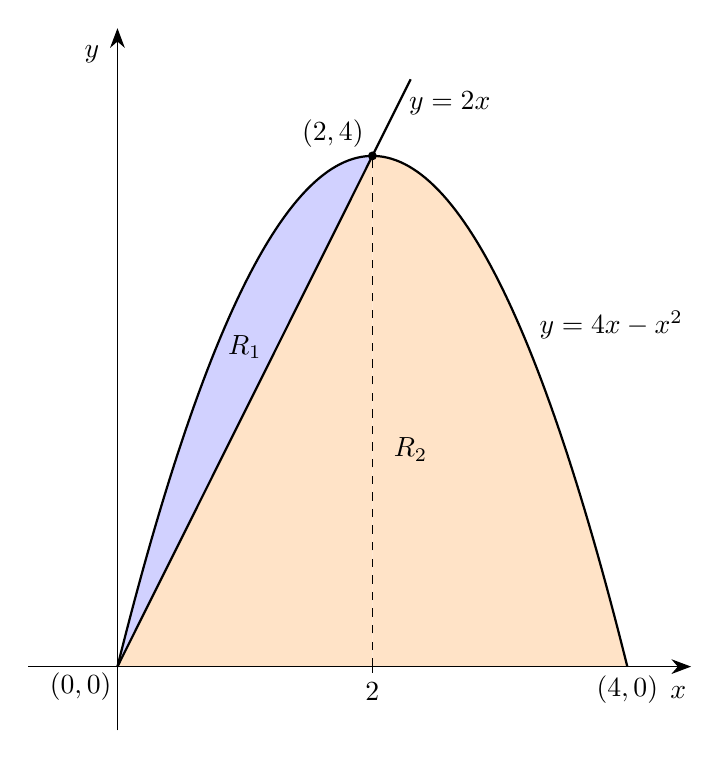
\begin{tikzpicture}
\pgfplotsset{compat=1.18}
\begin{axis}[
    width=10cm,
    height=10.5cm,
    xmin=-0.7, xmax=4.5,
    ymin=-0.5, ymax=5,
    axis lines=middle,
    axis line style={-{Stealth[length=2.5mm]}},
    axis on top,
    xtick={2},
    xticklabels={$2$},
    xtick style={black, thin},
    ytick=\empty,
    clip=true,
    samples=120
]
% Exact paths used to shade R_1.
\addplot[draw=none, name path=rOneCurve, domain=0:2]
    {4*x-x^2};
\addplot[draw=none, name path=rOneLine, domain=0:2, samples=2]
    {2*x};
\addplot[blue!18, draw=none]
    fill between[of=rOneCurve and rOneLine];

% Exact component paths used to shade R_2.
\addplot[draw=none, name path=rTwoLine, domain=0:2, samples=2]
    {2*x};
\addplot[draw=none, name path=rTwoAxisA, domain=0:2, samples=2]
    {0};
\addplot[orange!22, draw=none]
    fill between[of=rTwoLine and rTwoAxisA];

\addplot[draw=none, name path=rTwoCurve, domain=2:4]
    {4*x-x^2};
\addplot[draw=none, name path=rTwoAxisB, domain=2:4, samples=2]
    {0};
\addplot[orange!22, draw=none]
    fill between[of=rTwoCurve and rTwoAxisB];

% Boundary curve and dividing line, unchanged from the question.
\addplot[thick, black, domain=0:4]
    {4*x-x^2}
    node[pos=0.72, above right] {$y=4x-x^2$};
\addplot[thick, black, domain=0:2.3, samples=2]
    {2*x}
    node[pos=0.96, right] {$y=2x$};

% Region and axis labels, unchanged from the question.
\node at (axis cs:1,2.5) {$R_1$};
\node at (axis cs:2.3,1.7) {$R_2$};
\node at (axis cs:4.4,-0.2) {$x$};
\node at (axis cs:-0.2,4.8) {$y$};

% Exact intersection, integration boundary, and coordinate labels.
\coordinate (Origin) at (axis cs:0,0);
\coordinate (RightIntercept) at (axis cs:4,0);
\coordinate (Intersection) at (axis cs:2,4);
\coordinate (BoundaryFoot) at (axis cs:2,0);
\draw[thin, black, dashed] (BoundaryFoot) -- (Intersection);
\fill[black] (Intersection) circle[radius=1.6pt];
\node[below left, inner sep=2pt] at (Origin) {$(0,0)$};
\node[below, inner sep=3pt] at (RightIntercept) {$(4,0)$};
\node[above left, inner sep=3pt] at (Intersection) {$(2,4)$};
\end{axis}
\end{tikzpicture}
% end q000622 figure F1
\end{djsSolutionFigure}

The diagram shows that $R_1$ lies between the curve and line for $0\leq x\leq2$, while the whole region $R$ extends from $x=0$ to $x=4$.

For an upper curve $y=f(x)$ and a lower curve $y=g(x)$, the area between them from $x=a$ to $x=b$ is
\[
\text{Area}=\int_a^b\bigl(f(x)-g(x)\bigr)\,\mathrm{d}x
\]

For $R_1$, subtract the line's height from the curve's height:
\[
\begin{aligned}
\text{Area}(R_1)
&=\int_0^2\bigl((4x-x^2)-2x\bigr)\,\mathrm{d}x\\[8pt]
&=\int_0^2(2x-x^2)\,\mathrm{d}x\\[8pt]
&=\left[x^2-\frac{x^3}{3}\right]_0^2
=4-\frac83=\frac43
\end{aligned}
\]

For the whole region $R$:
\[
\begin{aligned}
\text{Area}(R)
&=\int_0^4(4x-x^2)\,\mathrm{d}x\\[8pt]
&=\left[2x^2-\frac{x^3}{3}\right]_0^4
=32-\frac{64}{3}=\frac{32}{3}
\end{aligned}
\]

Obtain the area of $R_2$ by subtraction, avoiding separate integrals on either side of $x=2$:
\[
\text{Area}(R_2)=\text{Area}(R)-\text{Area}(R_1)
=\frac{32}{3}-\frac43=\frac{28}{3}
\]

The required ratio is therefore
\[
\frac43:\frac{28}{3}=4:28=\boxed{1:7}
\]

The correct option is \textbf{C}.
% end q000622 solution
\end{djsSolution}
\end{enumerate}
\clearpage
\thispagestyle{djssolutions}
\vspace*{8pt}
\djsTopicLine{Exponentials \& Logarithms}
\begin{enumerate}[label=\textbf{\arabic*.},leftmargin=*,itemsep=0pt,start=19]
\questionitem[Exponentials \& Logarithms]
% begin q000728 stem
The curve $C$ has equation
\[\log_2(2y+4)=2\log_2(x+1)\]

For which values of the real constant $m$ does the line $y=mx$ meet $C$ at exactly two distinct points?
% end q000728 stem

\par\vspace*{12pt}
\begin{tabularx}{\linewidth}{@{}>{\bfseries}l Y@{}}
A &
% begin q000728 choice A
$m<2$
% end q000728 choice A
\\[0.8em]
B &
% begin q000728 choice B
$m\le 2$
% end q000728 choice B
\\[0.8em]
C &
% begin q000728 choice C
$m>0$
% end q000728 choice C
\\[0.8em]
D &
% begin q000728 choice D
$m>2$
% end q000728 choice D
\\[0.8em]
E &
% begin q000728 choice E
$m\ge 2$
% end q000728 choice E
\\
\end{tabularx}

\begin{djsSolution}{D}
% begin q000728 solution
First record the logarithm domains:
\[
x+1>0\quad\text{and}\quad 2y+4>0
\implies x>-1\quad\text{and}\quad y>-2
\]

Using the power law and then exponentiating with base $2$ gives
\[
\log_2(2y+4)=\log_2\bigl((x+1)^2\bigr)
\implies 2y+4=(x+1)^2
\]

To keep track of the restriction $x>-1$, put $u=x+1$, so $u>0$ and $x=u-1$. At an intersection with $y=mx$,
\[
u^2=2m(u-1)+4
\implies u^2-2mu+2m-4=0
\]

The discriminant is
\[
(-2m)^2-4(1)(2m-4)
=4m^2-8m+16
=4\bigl((m-1)^2+3\bigr)>0
\]

Thus this quadratic always has two distinct real roots, but we need both roots to be positive.

For a quadratic $au^2+bu+c=0$, the sum of the roots is $-b/a$ and their product is $c/a$. Here,
\[
\text{sum of roots}=2m
\qquad\text{and}\qquad
\text{product of roots}=2m-4
\]

Both roots are positive exactly when their sum and product are positive. A positive product makes the two real roots have the same sign, and a positive sum then makes both positive.
\[
2m>0\quad\text{and}\quad 2m-4>0
\iff m>0\quad\text{and}\quad m>2
\iff \boxed{m>2}
\]

The other logarithm domain is then automatic: each positive root gives $2y+4=u^2>0$. The two distinct values of $u$ give two distinct values of $x$, so the correct option is \textbf{D}.\\[5pt]

\textit{Alternative Solution:} (Testing the options)

To rule out a proposed range, choose a value of $m$ that it includes and show that the line has fewer than two intersections. Testing $m=0$ and $m=2$ distinguishes the options.

For $m=0$, the intersection quadratic found above factorises as
\[
u^2-4=0
\implies (u-2)(u+2)=0
\implies u=2\quad\text{or}\quad u=-2
\]

The root $u=-2$ is outside the domain $u>0$, so only $u=2$ is valid, giving the single intersection $(x,y)=(1,0)$. Both A and B include $m=0$, so both are ruled out.

For $m=2$, taking out the common factor $u$ gives
\[
u^2-4u=0
\implies u(u-4)=0
\implies u=0\quad\text{or}\quad u=4
\]

The root $u=0$ is excluded because it gives $x=-1$, where $\log_2(x+1)$ is undefined. Only $u=4$ is valid, giving the single intersection $(x,y)=(3,6)$.

Both C and E include $m=2$, so both are ruled out. The only remaining option is \textbf{D}.
% end q000728 solution
\end{djsSolution}
\end{enumerate}
\clearpage
\thispagestyle{djssolutions}
\vspace*{8pt}
\djsTopicLine{Logic}
\begin{enumerate}[label=\textbf{\arabic*.},leftmargin=*,itemsep=0pt,start=20]
\questionitem[Logic]
% begin q000784 stem
For a real constant $a$, the function $f$ is defined for $x>0$ by $f(x)=\sqrt{x}+\dfrac{a}{\sqrt{x}}$

Consider the conditions
\[
\begin{array}{@{}ll@{}}
\textbf{I} & f'(4)>0 \\[5pt]
\textbf{II} & f(4)>f(1) \\[5pt]
\end{array}
\]

Which of the following describes the relationship between conditions I and II?
% end q000784 stem

\par\vspace*{12pt}
\begin{tabularx}{\linewidth}{@{}>{\bfseries}l Y@{}}
A &
% begin q000784 choice A
I is necessary but not sufficient for II.
% end q000784 choice A
\\[0.8em]
B &
% begin q000784 choice B
I is sufficient but not necessary for II.
% end q000784 choice B
\\[0.8em]
C &
% begin q000784 choice C
I is both necessary and sufficient for II.
% end q000784 choice C
\\[0.8em]
D &
% begin q000784 choice D
I is neither necessary nor sufficient for II.
% end q000784 choice D
\\[0.8em]
E &
% begin q000784 choice E
I and II cannot both be true.
% end q000784 choice E
\\
\end{tabularx}

\begin{djsSolution}{A}
% begin q000784 solution
Condition I is necessary for II if II cannot hold without I. Condition I is sufficient for II if I guarantees II.

Writing the square roots as fractional powers and differentiating gives
\[
\begin{aligned}
f(x)&=x^{1/2}+ax^{-1/2}\\[5pt]
f'(x)&=\frac12x^{-1/2}-\frac a2x^{-3/2}
\end{aligned}
\]

First express condition I as an inequality in $a$:
\[
f'(4)=\frac12(4^{-1/2})-\frac a2(4^{-3/2})
=\frac14-\frac a{16}=\frac{4-a}{16}
\]

Hence condition I is equivalent to
\[
\frac{4-a}{16}>0\iff\boxed{a<4}
\]

Now express condition II as an inequality in $a$. The function values are
\[
f(4)=2+\frac a2
\qquad\text{and}\qquad
f(1)=1+a
\]

Therefore condition II is equivalent to
\[
2+\frac a2>1+a
\iff 1>\frac a2
\iff\boxed{a<2}
\]

For necessity, the required statement is: if $a<2$, then $a<4$. Every value below $2$ is also below $4$, so I is necessary for II.

For sufficiency, the required statement is: if $a<4$, then $a<2$. This fails at $a=2$, since
\[
\begin{aligned}
f'(4)&=\frac{4-2}{16}=\frac18>0\\[8pt]
f(4)&=2+\frac22=3\\[8pt]
f(1)&=1+2=3
\end{aligned}
\]

Thus I holds, but II does not: the two function values are equal rather than satisfying the strict inequality.

Condition I is necessary but not sufficient for II, so the correct option is \textbf{A}.
% end q000784 solution
\end{djsSolution}
\end{enumerate}
\end{document}
